\chapter{Procedimiento y descripción de las actividades realizadas}
Las actividades que en esta sección son descritas están redactadas en orden cronológico y con base en el cronograma de actividades. Es importante destacar que el cronograma de actividades fue elaborado de acuerdo al tablero de actividades Kanban que se realizó para dar seguimiento a todas las actividades que se han realizado para el desarrollo del proyecto.
    \section{Conociendo Mezfer Rewards}
Mezfer Rewards es un programa de recompensas creado por la compañía Mezfer para poder entregar a sus clientes diferentes premios mediante el canje de puntos que obtienen gracias a la compra de productos. Para poder llevar a cabo este programa, Mezfer decidió crear una aplicación web y una aplicación móvil.

Para poder comenzar con el nuevo proyecto ``Mezfer Insider'' fue de gran importancia conocer ambas aplicaciones con las que funciona el proyecto, pues estas sirven como antecedentes y guías para tener una idea más sólida sobre como se va a estructurar el nuevo proyecto y todas las funciones que se van a mantener o eliminar. 

A continuación, se describen de manera general ambas aplicaciones.
    \subsection{Aplicación web de Mezfer Rewards}
La aplicación web fue desarrollada utilizando Laravel, un framework para el lenguaje de programación PHP. Esta aplicación es un pánel de administración, por lo que sólo está pensada para ser utilizada por usuarios que sean administradores. 

La aplicación está integrada a un sistema más grande llamado ``Siso ERP'', un sistema integral de gestión empresarial que controla, facilita y optimiza los procesos operativos de las empresas. Por lo tanto, para poder acceder al pánel de administración de Mezfer Rewards, es necesario tener una cuenta en Siso ERP.

Una vez que el administrador ha ingresado, podrá realizar todas las acciones necesarias para gestionar el programa. Entre las acciones más importantes se encuentran: 
\begin{itemize}
    \item Gestión de usuarios: El administrador es capaz de activar o desactivar la cuenta de un usuario, modificar su rol y suscribir o desuscribir al usuario de una campaña.
    \item Gestión de campañas: El administrador es capaz de modificar toda la información relevante de una campaña como su descripción, los productos participantes y los premios disponibles.
    \item Gestión de solicitudes de puntos: El administrador es capaz de aceptar o rechazar una solicitud de puntos que haya enviado un cliente, de acuerdo a si la evidencia que envió es válida o no. 
\end{itemize}
Hay muchas más acciones que puede realizar el administrador y que complementan al programa de recompensas. Si bien son acciones que también son importantes, no es fundamental describirlas para poder comprender mejor la aplicación.
    \subsection{Aplicación móvil de Mezfer Rewards}
La aplicación móvil fue desarrollada con Flutter, un framework que permite desarrollar aplicaciones nativas para iOS y Android, y cuyo lenguaje de programación es Dart. Esta fue desarrollada específicamente para los clientes.

Al descargar e iniciar la aplicación, los clientes deberán ingresar su número telefónico y su contraseña para acceder; si no tienen cuenta, tendrán que registrarse.

Cuando el cliente ha iniciado sesión, accederá a la aplicación y podrá ver las campañas disponibles, así como otro contenido que podría ser de su interés. Es importante mencionar que la aplicación no cuenta con una función para inscribirse a la campaña que desee, pero esto no es una falla en el diseño, sino una decisión de la propia empresa; para que el cliente pueda inscribirse tendrá que comunicarse con un encargado de Mezfer y realizar la solicitud.

Si el cliente no está inscrito a ninguna campaña, sólo podrá revisar la información general como la descripción, los productos participantes y los premios disponibles; si el cliente está inscrito a alguna campaña, además de poder ver la información general, podrá realizar dos acciones más:
\begin{itemize}
    \item Realizar solicitud de puntos: El cliente es capaz de enviar una solicitud de puntos, en donde especifica los productos que compró y la cantidad, así como la evidencia de la compra.
    \item Canjear puntos disponibles: El cliente es capaz de canjear los puntos que obtuvo con la compra de productos para poder obtener premios que sean de su interés.
\end{itemize}
Hay otras acciones que puede realizar el cliente y que complementan su experiencia en el uso de la aplicación. Si bien son acciones que también son importantes, no es fundamental describirlas para poder comprender mejor la aplicación.
    \section{Análisis de la base de datos}
    \section{Selección de tecnologías a utilizar}
Como último paso para comenzar con el desarrollo de Mezfer Insider, se analizaron diferentes tecnologías para usar en frontend y backend.
    \subsection{Servicios en la nube}
La plataforma que se utilizó para proveer los servicios en la nube fue Amazon Web Services. De esta plataforma se utilizaron servicios como:
\begin{itemize}
    \item Amazon Elastic Compute Cloud (EC2): Es un servicio que proporciona capacidad de computación escalable bajo demanda en la nube. Permite lanzar cuantos servidores virtuales sean necesarios. Dos instancias de EC2 fueron utilizadas para lanzar el proyecto de Mezfer Insider y la API.
    \item Amazon Relational Database Service (RDS): Es un servicio web que facilita la configuración, la operación y la escala de una base de datos relacional en la nube. Se utilizó este servicio para crear la base de datos de Mezfer Insider.
    \item Amazon Simple Storage Service (S3): Es un servicio de almacenamiento de objetos que ofrece escalabilidad, disponibilidad de datos, seguridad y rendimiento líderes del sector. Este servicio fue utilizado para almacenar recursos importantes de Mezfer Insider, como archivos e imágenes.
\end{itemize}
    \subsection{Tecnologías de frontend}
Para facilitar el desarrollo del frontend, se decidió comprar una plantilla de pánel de usuario llamada DashTail, la cual proporciona vistas ya diseñadas o componentes para poder ir construyendo poco a poco la vista para el usuario; esta plantilla ofrece una alta personalización, por lo que es posible realizar cualquier cambio a los componentes.

DashTail fue desarrollada utilizando Next.js y Tailwind CSS. 

Next.js es un framework basado en JavaScript y React que permite crear aplicaciones web modernas, dinámicas y escalables. Aunque es un framework full-stack, en DashTail sólo se utiliza para frontend.

Tailwind CSS es un framework de CSS para el diseño de páginas web. Su principal característica es que no genera una serie de clases predefinidas para elementos, en su lugar, crea una lista de clases ``de utilidad'' que son utilizas para dar estilos individuales a cada elemento. Es gracias a este framework que los componentes de la plantilla son altamente personalizables.
    \subsection{Tecnologías de backend}
El backend consistió en desarrollar una API para que el frontend pudiera comunicarse con esta y realizar peticiones HTTP para interactuar con la base de datos.

La principal tecnologia de backend es Node.js, un entorno de ejecución utilizado para poder ejecutar código de JavaScript directamente en los servidores, es decir, sin la necesidad de un navegador web.

Junto a Node.js se utiliza Express.js, un framework de backend para Node.js que proporciona características y herramientas robustas para desarrollar aplicaciones de backend escalables. Sus herramientas como peticiones y respuestas HTTP, enrutamiento y middlewares resultaron muy útiles para el desarrollo de la API.
    \section{Inicialización y despliegue de los proyectos de Frontend y Backend}
Para comenzar con el desarrollo de Mezfer Insider fue necesario crear los proyectos e instalar las dependencias necesarias para que estos funcionaran correctamente.
    \subsection{Inicialización del proyecto de Frontend}
Como se mencionó anteriormente, para el Frontend se utilizó una plantilla llamada DashTail, la cual proporciona un conjunto de páginas ya diseñadas. Esta plantilla es un proyecto de Next.js, por lo que, en este caso, no fue necesario crear el proyecto desde cero.

Para poder ejecutar el proyecto es necesario instalar todas las dependencias necesarias con el gestor de dependencias que se prefiera. En este proyecto se decidió utilizar el gestor de dependencias Yarn.

Cuando se instala Node.js, el gestor de dependencias predeterminado es NPM (Node Package Manager), por lo que si se desea utilizar Yarn será necesario realizar una instalación extra. En la página oficial de Yarn se explica de una manera breve y sencilla como se realizar la instalación; utilizando NPM se ejecuta el siguiente comando:
    \begin{center}
        \textbf{
            \emph{
                npm install --global yarn
                }
            }
    \end{center}
De esta manera Yarn quedará instalado en todo el sistema y podrá ser utilizado en cualquier proyecto.

Ahora, lo único que queda es instalar las dependencias del proyecto. Para esto, se ejecuta el comando: 
    \begin{center}
        \textbf{
            \emph{
                yarn install
                }
            }
    \end{center}
Y con esto comenzará la instalación.

Una vez instaladas todas las dependencias, se ejecuta el comando:
    \begin{center}
        \textbf{
            \emph{
                yarn dev
                }
            }
    \end{center}
Esto iniciará el entorno de desarrollo del proyecto, que será ejecutado en un servidor local y para acceder a él simplemente en un navegador escribimos la URL \emph{http://localhost:3000} (El puerto 3000 es el puerto predeterminado en el cual se ejecuta el servidor local de Next.js, sin embargo, este puede ser cambiado al puerto que se desee).
    \subsection{Despliegue del proyecto de Frontend en servidor de producción}
Para desplegar el proyecto en el servidor de producción se deben seguir casi los mismos pasos que con la inicialización, pero hay algunos pasos extra que deben realizarse.

Principalmente, deben de estar instalados Node.js y Yarn para poder instalar las dependencias y ejecutar el proyecto. El proceso de instalación es el mismo, no hay ninguna diferencia.

Otra herramienta importante que se debe instalar es PM2 (Process Manager 2), un gestor de procesos que permite mantener proyectos de Node.js en ejecución, es decir, si el servidor llegase a ser detenido o reiniciado, PM2 se encargará de iniciar el proyecto automáticamente sin la necesidad de que un administrador ingrese al servidor a iniciar todos los proyectos nuevamente. Para instalar PM2, se ejecuta el siguiente comando:
    \begin{center}
        \textbf{
            \emph{
                yarn global add pm2
                }
            }
    \end{center}
El siguiente paso es compilar el proyecto para que Next.js realice todas las optimizaciones necesarias y así quede preparado para producción. Para compilar el proyecto, desde la carpeta principal se ejecuta el siguiente comando:
    \begin{center}
        \textbf{
            \emph{
                yarn build
                }
            }
    \end{center}
De esta manera Next.js comenzará a compilar y optimizar todas las páginas que tenga la aplicación. Al finalizar el proceso, se creará una carpeta llamada ``.next'', la cual contiene el proyecto optimizado y listo para producción.

Ahora, hay 5 archivos importantes que deben ser enviados al servidor para poder ejecutar correctamente el proyecto:
    \begin{itemize}
        \item .next: Esta es la carpeta que contiene todo el proyecto optimizado.
        \item .env: Este es el archivo donde se almacenan las variables de entorno.
        \item package.json: Este es el archivo que contiene todas las dependencias que han sido instaladas en el proyecto.
        \item yarn.lock: Un archivo generado por Yarn que lleva un registro de las versiones exactas de las dependencias que requiere un proyecto para que funcione adecuadamente.
        \item next.config.js: Este es el archivo que contiene la configuración del servidor de Next.js.
    \end{itemize}
Para enviar estos archivos al servidor, se ejecuta el siguiente comando:
    \begin{center}
        \textbf{
            \emph{
                scp -i --/ruta/llave/PEM -r archivos usuario@ip\_{}publica\_{}servidor:--/carpeta/destino
                }
            }
    \end{center}
Una vez estén todos los archivos en el servidor de producción, se instalan las dependencias como se explicó anteriormente, y finalmente, se ejecuta el proyecto con PM2 para que este se encargue de gestionarlo. Para ejecutar el proyecto con PM2, se utiliza el siguiente comando:
    \begin{center}
        \textbf{
            \emph{
                pm2 start ``yarn start'' --name nombre-app
                }
            }
    \end{center}
Posteriormente, se guarda la configuración con el siguiente comando:
    \begin{center}
        \textbf{
            \emph{
                pm2 save
                }
            }
    \end{center}
Para hacer que la aplicación se ejecute automáticamente cuando se reinicie el servidor, se utiliza el siguiente comando:
    \begin{center}
        \textbf{
            \emph{
                pm2 startup
                }
            }
    \end{center}
Al ejectuar este comando PM2 proporcionará otro comando que solamente debe ser copiado, pegado y ejecutado, y se habrá terminado de configurar. Ahora, con cada reinicio del servidor, la aplicación se ejecutará automáticamente.

Cuando se quieran subir cambios al proyectos, simplemente se repiten los pasos:
    \begin{itemize}
        \item Compilar el proyecto.
        \item Subir los archivos que hayan sufrido cambios al servidor.
        \item Reiniciar el proceso de PM2.
    \end{itemize}
Para reiniciar el proceso de PM2, se ejecuta uno de los siguientes comandos:
    \begin{center}
        \textbf{
            \emph{
                pm2 reload nombre-app
                }
            }

        \textbf{
            \emph{
                pm2 restart nombre-app
            }
        }
    \end{center}
Y con esto quedarán aplicados los cambios que se hayan subido.
    \subsection{Inicialización del proyecto de Backend}
El proyecto de Backend consiste en una API realizada en el framework Express.js. Este proyecto sí es creado desde cero, por lo que se deben seguir unos cuantos pasos extra. Es importante mencionar que también debe estar ya instalado Node.js, al igual que un gestor de dependencias.

Lo primero que se tiene que hacer es crear una carpeta donde va a estar guardado todo el proyecto. Para crear una carpeta, se ejecuta el siguiente comando (puede cambiar de acuerdo al Sistema Operativo que se use):
    \begin{center}
        \textbf{
            \emph{
                mkdir nombre-carpeta
                }
            }
    \end{center}
Posteriormente, se ingresa a la carpeta y desde ahí se ejecuta el siguiente comando:
    \begin{center}
        \textbf{
            \emph{
                npm init -y
                }
            }
    \end{center}
Lo que hace ese comando es iniciar la configuración del proyecto, al usuario se le hacen ciertas preguntas para saber que cosas quiere incluir o usar. La opción -y hace que a todas las preguntas se les responda con un ``sí'', por lo que se puede omitir si se desea pensar un poco más en la configuración.

Como esta es una API realizada con Express.js, es necesario instalar el paquete. Para instalar Express.js, se ejecuta el siguiente comando:
    \begin{center}
        \textbf{
            \emph{
                npm install express
                }
            }
    \end{center}
Ahora sólo falta crear el servidor de Express, ya que ahí es donde se realizarán las diferentes solicitudes HTTP desde el Frontend. Para lograr esto, se crea un archivo que preferentemente se llame ``index.js'', aunque puede llevar cualquier nombre; en este archivo es donde se inicializa el servidor y se colocan las rutas y middlewares que vayan a ser ocupados. Para inicializar el servidor de Express, se añaden las siguientes líneas de código (Ver figura 1):

    \begin{figure}[H]
        \begin{center}
            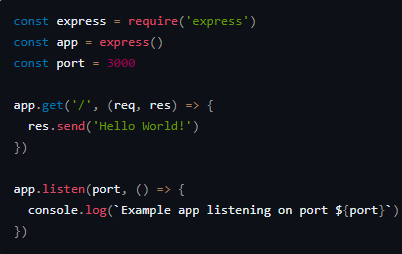
\includegraphics[scale=0.84]{img/actividades/inicializacion-despliegue/express-basic-app.png}
            \caption{Aplicación básica de Express.}
            \label{fig:express-basic-app}
        \end{center}
    \end{figure}
Y para ejecutar la aplicación, se utiliza el siguiente comando:
    \begin{center}
        \textbf{
            \emph{
                node index.js
                }
            }
    \end{center}
Con ese comando se ejecuta el servidor de manera local y se pueden realizar algunas solicitudes HTTP a la URL \emph{http://localhost:3000}.
    \subsection{Despliegue del proyecto de Backend en servidor de producción}
La estrategia que se siguió para desplegar la API en el servidor de producción fue utilizar repositorios de GitHub, ya que estos es posible clonarlos en cualquier parte y esto facilita y simplifica el proceso de despliegue.

Lo primero que se debe hacer es crear un repositorio de GitHub. Esto se puede hacer desde la línea de comandos o desde la página web, pero para más facilidad se recomienda realizarlo desde la página web. Una vez creado el repositorio, se proporcionan una serie de comandos que se deben ejecutar para inicializar el repositorio local y subir el código ya existente al repositorio remoto.

Una vez que el código se encuentre en el repositorio remoto sigue clonarlo en el servidor de producción. Realizar la clonación de un repositorio es muy sencillo, sólo es necesario ingresar al servidor y ubicarse en el directorio donde va a estar el proyecto, luego se ejecuta el siguiente comando: 
    \begin{center}
        \textbf{
            \emph{
                git clone ruta-del-repositorio-remoto
                }
            }
    \end{center}
Y con esto todas las carpetas y archivos del proyecto estarán en el servidor de producción. Después, se deben instalar todas las dependencias mediante el siguiente comando:
    \begin{center}
        \textbf{
            \emph{
                npm install 
                }
            }
    \end{center}
El último paso es hacer que se ejecute automáticamente la aplicación, y esto se logra gracias a PM2. Los comandos que se utilizan son prácticamente los mismos, sólo hay una ligera variación en el primer comando que se utiliza, puesto que ejectuar una aplicación de Express es diferente a ejecutar una aplicación de Next.js. El comando que se debe usar para esta aplicación es el siguiente:
    \begin{center}
        \textbf{
            \emph{
                pm2 start ``node index.js'' --name nombre-app
                }
            }
    \end{center}
Los siguientes comandos a ejecutar son exactamente los mismos que se explicaron en el despliegue de la aplicación del Frontend.

Para actualizar la aplicación, simplemente se suben los cambios realizados en el código al repositorio remoto y se descargan en el servidor de producción mediante el siguiente comando:
    \begin{center}
        \textbf{
            \emph{
                git pull
                }
            }
    \end{center}
Una vez descargados los cambios, se reinicia el proceso de PM2 y la aplicación ya estará en su última versión.
    \section{Creación de balanceadores de carga y asignación de los dominios}
    \section{Integración de Mezfer Insider con Control Manager Siso}
Control Manager Siso (CMS) es el sistema de inicio de sesión de Siso ERP, un sistema ERP que permite realizar la gestión de distintos aspectos de una empresa. Cuando un cliente compra una licencia de Siso ERP, se le otorgan un correo y contraseña que podrán usar para iniciar sesión mediante CMS y acceder a sus empresas.

Quienes son administradores de CMS tienen acceso al panel de administración, donde se les permite gestionar a los usuarios y empresas del sistema Siso ERP.

Para poder crear empresas (que son tratadas como aplicaciones web), CMS realiza peticiones a diferentes endpoints de la API de la nueva empresa y, dependiendo de la respuesta que se reciba, se registrará correctamente a la base de datos o no. Lo mismo aplica para cuando se quiere asignar un usuario a una empresa y cuando se quiere ingresar a la empresa.
    \subsection{Creación de endpoints en la API de Mezfer Insider}
En la API de Mezfer Insider deben existir tres endpoints que permitirán a CMS realizar las acciones necesarias para registrar el proyecto en su base de datos.

El primer endpoint consiste en que se procese la información de la empresa. Mediante el Frontend, el administrador ingresa la información de la empresa en el formulario correspondiente y esta es enviada a la API; dependiendo de las necesidades del proyecto, esta información puede ser procesada o solamente recibida. En el caso de Mezfer Insider, esta información no requiere ser almacenada ni requiere ser procesada. Se debe retornar una respuesta con el código de estado de respuesta HTTP 202, indicando así que la petición se ha recibido, pero no se ha actuado.

El segundo endpoint consiste en vincular a un usuario con la empresa para indicar al sistema que ese usuario va a poder acceder a la empresa. En CMS, el administrador se encargará de asignarle la empresa al usuario, lo que enviará una nueva petición a la API para permitir la vinculación. La API recibirá el usuario y la empresa que están siendo vinuclados, esta información será procesada de acuerdo a las necesidades del proyecto. La API enviará un código de estado de respuesta HTTP 200, indicando que la operación ha sido realizada con éxito.

El tercer endpoint permitirá al usuario acceder a la empresa. Este endpoint es un poco más complejo, pues requiere el procesamiento de tokens JWT. Cuando el usuario ingresa en la empresa, CMS envía en la URL un token JWT con cierta información del usuario.
Para Mezfer Insider, esta información es importante pues se considera que todos los usuarios que ingresen mediante CMS son administradores, así que debe de quedar registro de ellos. Cuando se recupera el token de la URL, este es decodificado y se lee cierta información que posteriormente es utilizada para realizar otra petición a la API de CMS y así obtener la información completa del usuario; con esto se crea un objeto con la información que se requiere del usuario para guardarla en la base de datos. Una vez guardado el usuario, se procede a crear un token JWT propio de Mezfer Insider que posteriormente será almacenado en una cookie, de esta manera se creará una cookie de sesión que será de utilidad para permitir al usuario realizar distintas acciones dentro de la aplicación. Este proceso se repite cada que un usuario ingresa a la empresa, por lo que debe validarse la existencia del usuario en la base de datos para evitar que se intente guardar nuevamente.
    \subsection{Creación de la empresa, vinculación del usuario e ingreso}
Con los endpoints creados, ya es posible realizar todas las acciones necesarias para integrar Mezfer Insider con CMS.

Lo primero que se tiene que hacer es crear la empresa, y para eso se llena un formulario con todos los datos de la empresa.
    \begin{figure}[H]
        \begin{center}
            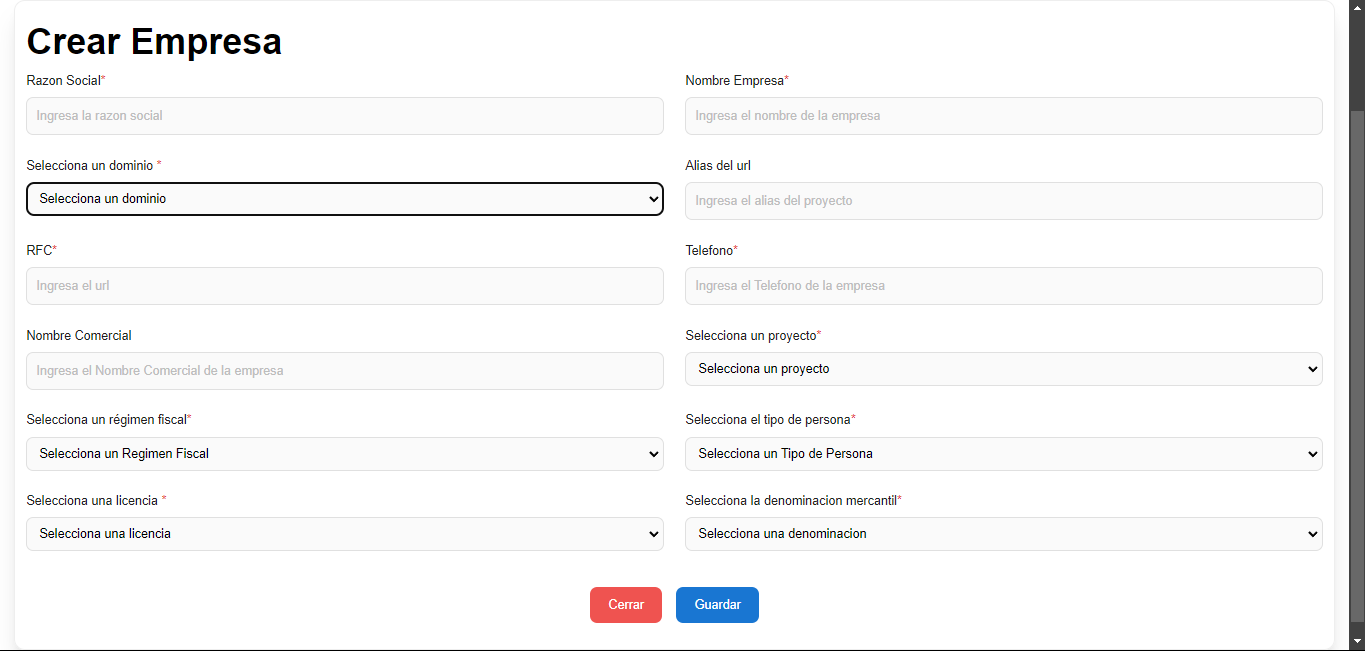
\includegraphics[scale=0.4]{img/actividades/integracion/formulario-empresa.png}
            \caption{Formulario para la creación de empresa.}
            \label{fig:formulario-empresa}
        \end{center}
    \end{figure}
Posteriormente, el usuario debe ser vinculado con la empresa.
    \begin{figure}[H]
        \begin{center}
            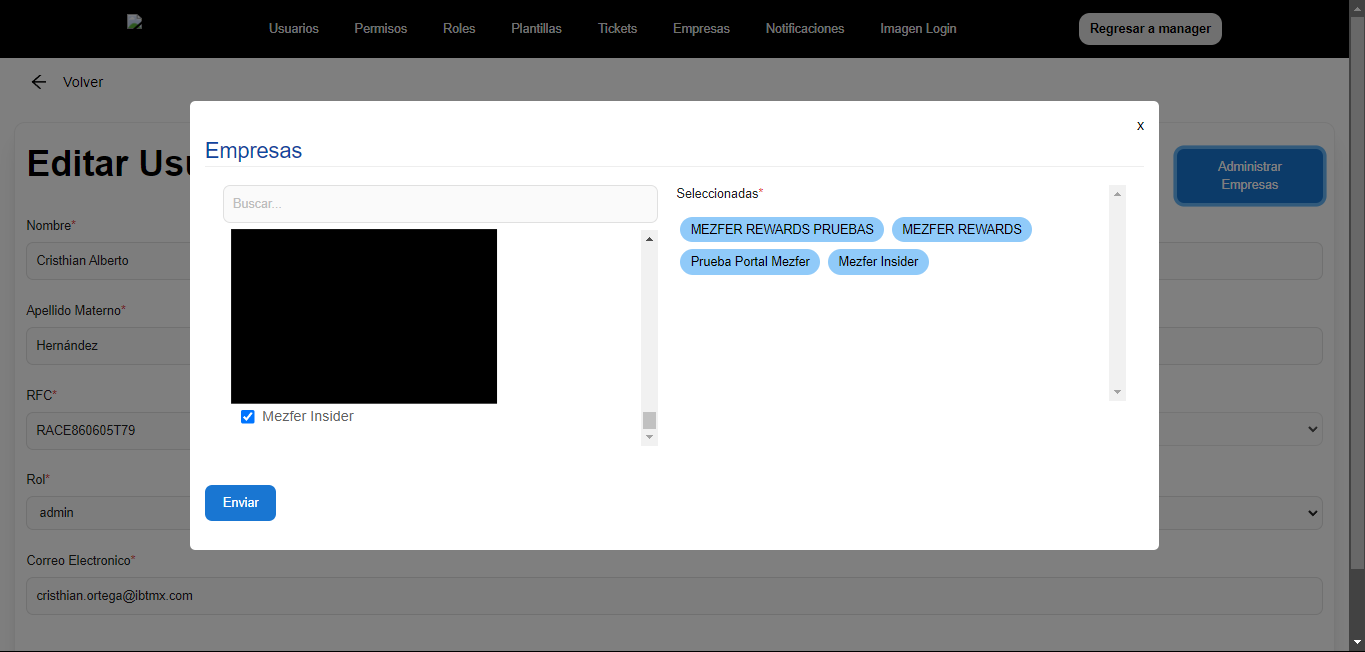
\includegraphics[scale=0.4]{img/actividades/integracion/vincular-usuario.png}
            \caption{Vinculación de usuario con empresa.}
            \label{fig:vincular-usuario}
        \end{center}
    \end{figure}
Y con esto realizado, el usuario ya podrá tener acceso a la empresa.
    \begin{figure}[H]
        \begin{center}
            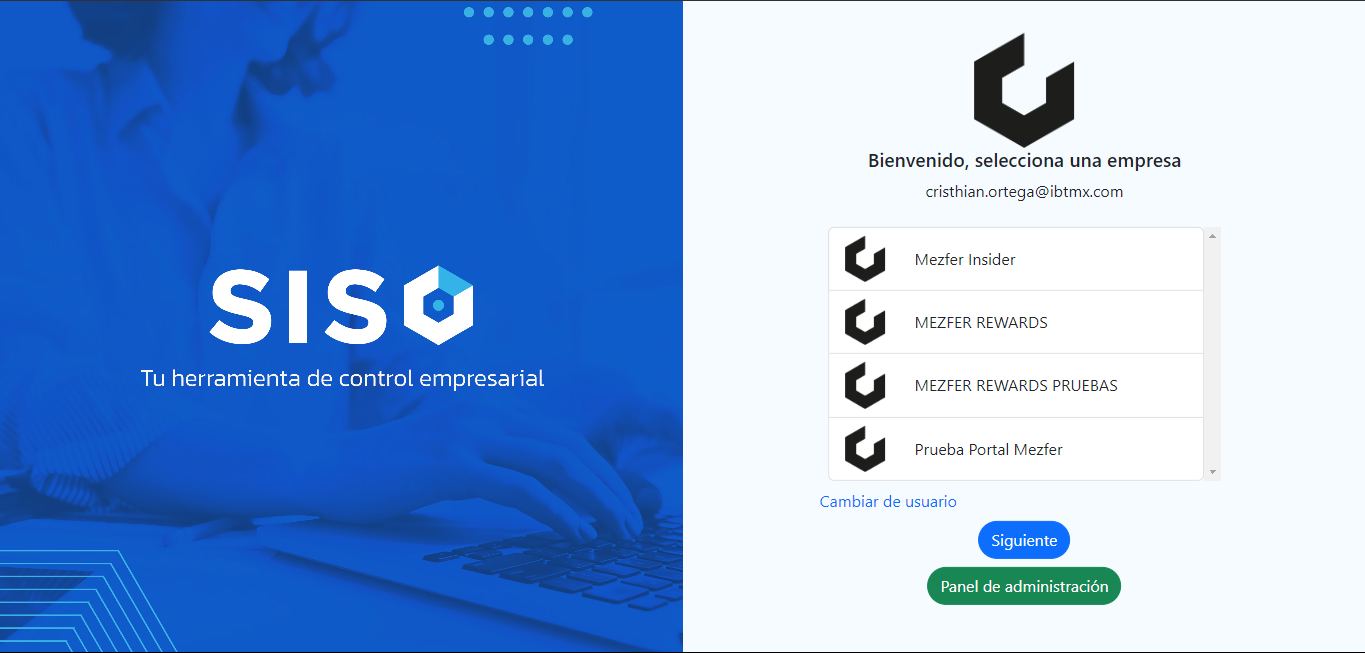
\includegraphics[scale=0.4]{img/actividades/integracion/ingreso-empresa.png}
            \caption{Selección de empresa.}
            \label{fig:ingreso-empresa}
        \end{center}
    \end{figure}
    \section{Creación de conexiones a las bases de datos}
Para poder empezar a codificar todas las acciones que se podrán realizar en Mezfer Insider, es necesario que en el backend estén realizadas las conexiones a las bases de datos para poder recuperar y guardar información.

Se realizaron dos conexiones puesto que, hasta el momento de la redacción de este reporte, Mezfer Insider ocupaba tanto la antigua base de datos como la nueva.
    \subsection{Instalación de librería}
Para poder realizar las conexiones a las bases de datos es necesario instalar una librería que proporcione los módulos del Sistema Gestor de Bases de Datos.

La librería que se seleccionó para este proyecto fue Knex.js, un constructor de queries de código abierto para JavaScript. Knex.js tiene soporte para varios SGBD, incluído PostgreSQL, que es el que se utiliza.

Para instalar Knex.js, se ejecuta el siguiente comando dentro de la carpeta del proyecto:
    \begin{center}
        \textbf{
            \emph{
                npm install knex
                }
            }
    \end{center}
    \subsection{Configuración de conexiones}
Con Knex.js instalado, sólo falta configurar las conexiones.

Para realizar las configuraciones, se debe crear un archivo que lleve de preferencia el nombre ``knexfile.js''. En este archivo, se crea un objeto con las siguientes propiedades:
    \begin{itemize}
        \item alias: El nombre que se le dará a la conexión.
        \item client: El SGBD que se utilizará para realizar la conexión.
        \item connection: En esta propiedad se debe configurar lo siguiente:
            \begin{itemize}
                \item host: El servidor donde está almacenada la base de datos.
                \item port: El puerto donde se está ejecutando el SGBD.
                \item database: El nombre de la base de datos.
                \item user: El nombre del usuario dueño de la base de datos.
                \item password: La contraseña para acceder a la base de datos.
            \end{itemize}
        \item pool: En esta propiedad se debe configurar lo siguiente:
            \begin{itemize}
                \item min: El número mínimo de conexiones que se pueden realizar.
                \item max: El número máximo de conexiones que se pueden realizar.
                \item afterCreate: Una función que se ejecuta una vez realizada la conexión. Esta es opcional
            \end{itemize}
    \end{itemize}
La estructura del objeto queda de la siguiente manera (Ver Figura 5):
    \begin{figure}[H]
        \begin{center}
            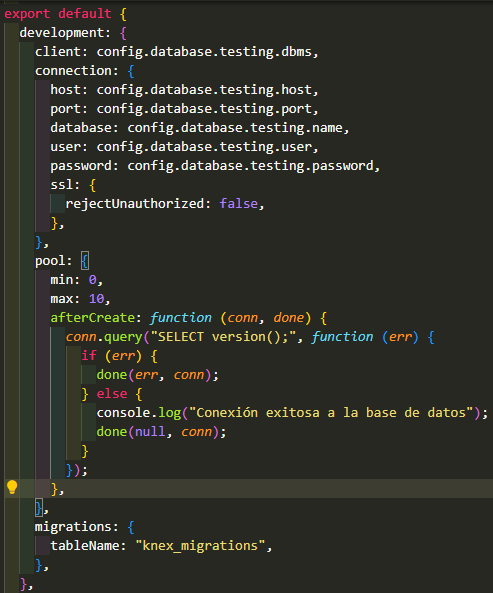
\includegraphics[scale=0.6]{img/actividades/conexion/objeto-conexion.png}
            \caption{Estructura del objeto de configuración de la conexión.}
            \label{fig:estructura-objeto}
        \end{center}
    \end{figure}
Por último, se crea una instancia de Knex y se le asigna la configuración que se desea utilizar, de esta manera se creará la conexión y se podrán realizar los queries que se requieran.
    \section{Inicio de sesión para Mezfer Insider}
El ingreso a Mezfer Insider se puede hacer de dos maneras: como cliente o como administrador.

En esta sección se explicará cómo se desarrollo el inicio de sesión de ambos roles.
    \subsection{Inicio de sesión de administradores}
Anteriormente se explicó una actividad donde se integraba Mezfer Insider a CMS. Esta integración, además de permitir la creación de la empresa en el sistema, también permite el inicio de sesión de los administradores pues todas las personas que ingresen a Mezfer Insider desde CMS son consideradas con ese rol.

Explicar como se realizó el inicio de sesión de administradores sería redundante, pues esto ya se explicó anteriormente. Para conocer este proceso, puede leer la sección 6.6 de este reporte.
    \subsection{Inicio de sesión de clientes}
Para la creación del inicio de sesión de clientes se realizaron actividades en el Frontend y en el Backend.
    \subsubsection{Endpoint de inicio de sesión}
El primer paso para la creación del endpoint del Backend es construir la query que permitirá buscar al cliente en la base de datos. Esta query es una busqueda en la tabla de clientes que recibe como parámetro ya sea el correo o el teléfono, y una vez encontrado, retorna toda la información.

Con la información del cliente recibida, se recupera la contraseña almacenada en la base de datos y se compara con la que se recibió desde el Frontend. Para realizar la comparación, es necesario desencriptar la contraseña de la base de datos, de esta manera se podrá saber si lo que ingresó el cliente es lo mismo que está en la base de datos.

Si las credenciales del cliente son correctas, se crea un token JWT con información útil del cliente y se almacena en una cookie de sesión.

Con este proceso realizado, el cliente podrá ingresar a Mezfer Insider.
    \subsubsection{Formulario de inicio de sesión}
Para que un cliente pueda iniciar sesión necesita de un formulario donde pueda ingresar sus datos como correo y contraseña.

El formulario que se creó está conformado por dos campos: en el primer campo se le solicita al cliente que ingrese su correo electrónico o su número de teléfono y en el segundo campo se le solicita su contraseña (Ver Figura 6).

    \begin{figure}[H]
        \begin{center}
            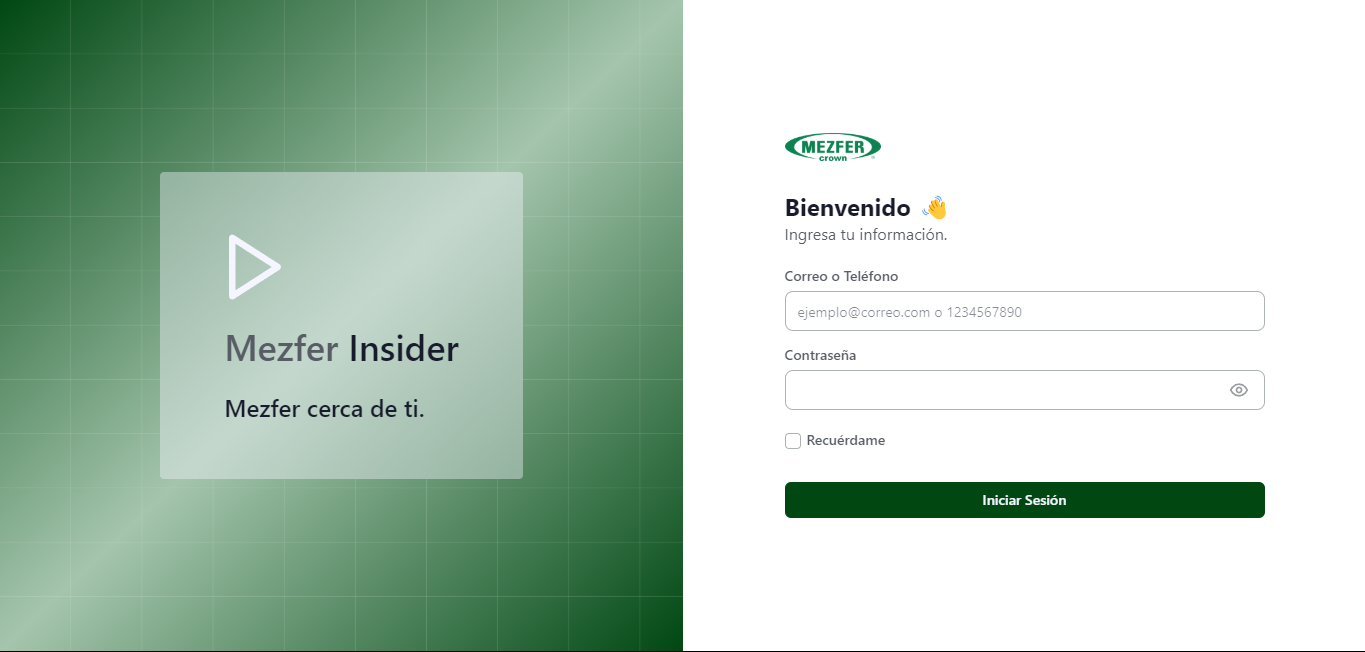
\includegraphics[scale=0.35]{img/actividades/login/Formulario-login.png}
            \caption{Formulario de inicio de sesión de clientes.}
            \label{fig:formulario-login}
        \end{center}
    \end{figure}

El campo de correo electrónico o teléfono está validado mediante expresiones regulares, de esta manera si el cliente escribe algo que no tenga la estructura de alguna de esas dos opciones, no podrá avanzar en el envío de la información. Además, esta validación también permite que el sistema detecte que opción de inicio de sesión se va a usar. Si la validación se cumple para correo electrónico, el objeto que se crea con la información de inicio de sesión del usuario sólo enviará correo y contraseña, y en el Backend se realizará la búsqueda del cliente mediante correo; si la validación se cumple para teléfono, el objeto sólo enviará teléfono y contraseña y se realizará la búsqueda del cliente mediante teléfono.

El cliente no podrá iniciar sesión hasta que ambos campos tengan información y esa información tenga el formato esperado.
    \section{Dashboard del cliente}
Hasta el momento de la redacción de este reporte, el dashboard del cliente sólo muestra un saludo personalizado y las campañas activas de Mezfer.
    \subsection{Endpoints del backend para el dashboard}
Para poder mostrar el contenido correcto en el dashboard, primero es necesario obtenerlo de la base de datos. Para ello, se crearon dos endpoints en la API.
    \subsubsection{Endpoint para obtener las campañas activas}
En la base de datos existe una tabla donde se almacenan todas las campañas activas y su información principal, y es necesario obtener esta información para poder mostrarla al usuario en el dashboard.

El endpoint que se debe crear es el que permite obtener las campañas disponibles. El query de este endpoint consiste en obtener todos los registros de la tabla de campañas

Cuando el Frontend realice la petición al Backend, este último le retornará un JSON con las campañas activas.
    \subsubsection{Endpoint para obtener la información del usuario}
Este endpoint permitirá obtener la información de un cliente de la tabla correspondiente en la base de datos.

Como en endpoints anteriores, lo primero que se tiene que hacer es crear el query que permita obtener la información. Es importante enviarle como parámetro el ID del cliente para que sólo se obtenga la información del cliente que se requiere y no se obtengan todos los registros existentes.

La obtención del ID se realiza con la ayuda del Frontend. Cada que se realice la petición HTTP a este endpoint se envían las credenciales, es decir, la cookie de sesión y esta será procesada por la API. La cookie contiene un token JWT con información del usuario, y entre esta información se encuentra el ID por lo que se debe extraer el token de la cookie, decodificarlo y obtener el ID para pasarlo al query.

Una vez ejecutado el query, el endpoint retornará un JSON con la información del cliente.
    \subsection{Interfaz del Dashboard}
Al iniciar sesión, la primera página que ve el cliente es el dashboard. En este dashboard se muestra un mensaje personalizado para el cliente y las campañas activas de Mezfer (Ver Figura 7).

    \begin{figure}[H]
        \begin{center}
            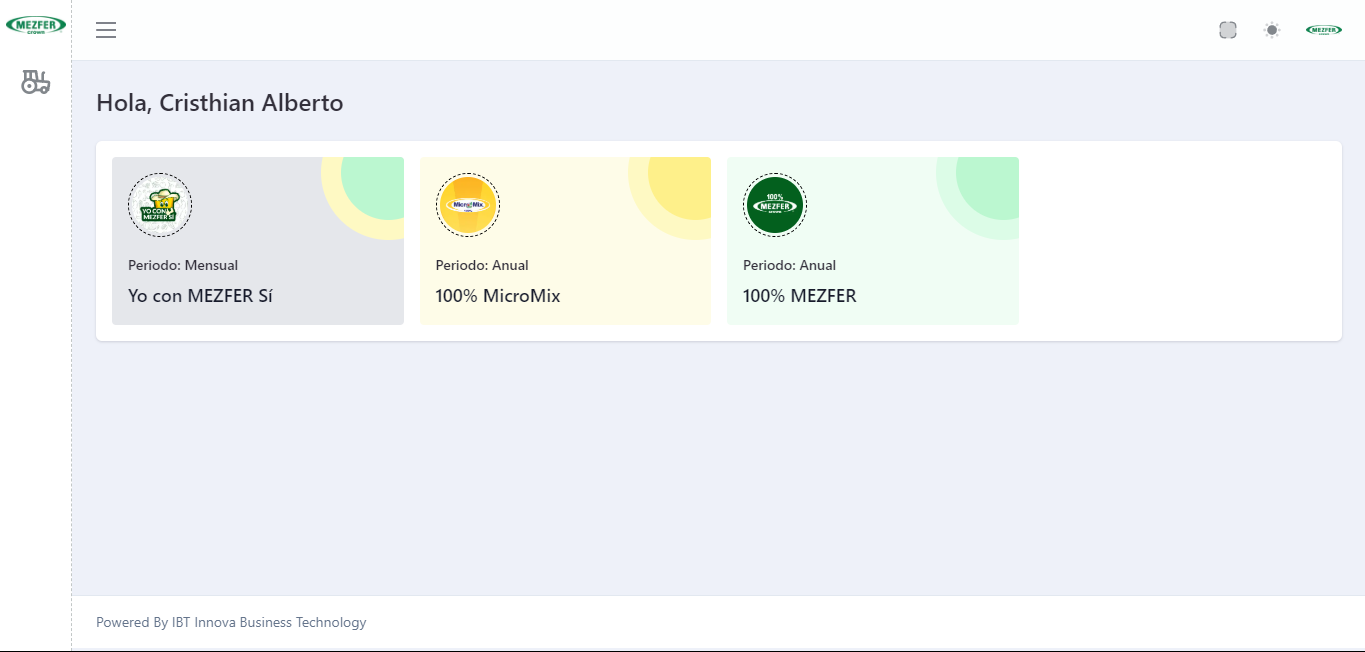
\includegraphics[scale=0.35]{img/actividades/dashboard-cliente/dashboard-cliente.png}
            \caption{Dashboard de clientes.}
            \label{fig:dashboard-clientes}
        \end{center}
    \end{figure}

Antes de cargar las campañas y el mensaje personalizado, se renderiza un componente llamado ``Skeleton'' que muestra la estructura de la página pero sin ningún contenido, sólo elementos grises que representan que la información se esta cargando. Este componente se muestra en lo que se obtiene la información de la API.

Una vez se haya cargado la información, el Skeleton deja de renderizarse y ahora muestra el mensaje personalizado y las campañas activas en componentes llamados ``Cards''. El cliente puede dar clic a cada una de estas Cards, lo que lo llevará a otra página donde se muestran todos los detalles de la campaña, pero esto se explicará más adelante.
    \section{Sección ``Mis campañas''}
La sección de campañas tiene un diseño muy similar al dashboard del clientes, lo que las hace diferentes es que la sección de campañas muestra en cuales se encuentra inscrito el usuario.
    \subsection{Endpoints del backend de la sección ``Mis campañas''}
La sección de campañas sólo requiere de dos endpoints: uno para obtener las campañas activas y otro para obtener las camapañas en las que está inscrito el usuario.
    \subsubsection{Endpoint para obtener las campañas activas}
Como se mencionó anteriormente, la interfaz de esta sección es muy similar a la del dashboard, por lo que comparten un mismo endpoint para obtener las campañas activas. Para saber como funciona este endpoint, puede leer la sección 6.9.1.1 de este documento.
    \subsubsection{Endpoint para obtener las campañas en las que se encuentra inscrito el usuario}
Para obtener la información que se requiere, se hará uso de la tabla que es producto de una relación muchos a muchos entre las tablas que contienen la información de los usuarios y de las campañas. Esta tabla intermedia permite relacionar un usuario con muchas campañas, permitiendo así que pueda estar inscrito en varias camapañas.

Se debe construir el query que permita obtener la información de la tabla correspondiente. Este query requiere del ID del usuario, para que sólo devuelva la información del usuario que se desea y no toda la información que contenga la tabla, además, también se debe verificar que el usuario siga inscrito en esta campaña; si no se valida esto, se obtendrán todas las campañas en las que ha estado el usuario, sin importar si sigue inscrito o no.

Con el query construido, al realizar la petición HTTP a este endpoint, se obtendrá un JSON con las campañas en las que está inscrito el usuario.
    \subsection{Interfaz de la sección ``Mis campañas''}
En la parte izquierda de la página web, el usuario podrá ver una barra de navegación que contiene un ícono de un tractor. Al dar clic en este tractor, el usuario será dirigido a la sección ``Mis campañas''.

En esta sección también se utiliza el componente ``Skeleton'' para indicar que se está cargando la información.

Cuando se cargan la información, el Frontend recibe todas las campañas activas y las campañas en las que se encuentra inscrito el usuario. Antes de construir la interfaz, se realiza un filtrado de los resultados obtenidos. Dentro del arreglo que contiene las campañas activas se buscan coincidencias con el arreglo que contiene las campañas en las que está inscrito el usuario; las campañas que se encuentren en ambos arreglos se almacenan en un nuevo arreglo, y las que no coincidan se ignoran.

Este nuevo arreglo es el que se utiliza para renderizar las Cards de las campañas, y de esta manera sólo se le muestran al usuario sus campañas correspondientes (Ver Figura 8).

    \begin{figure}[H]
        \begin{center}
            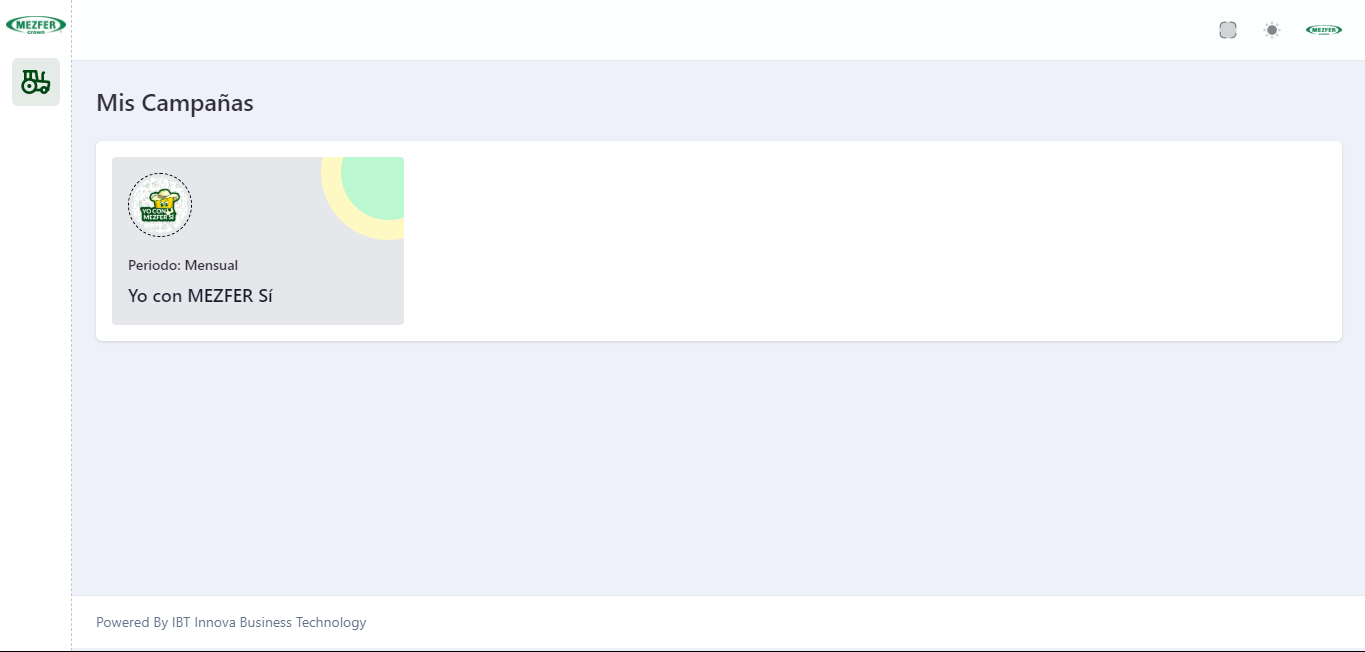
\includegraphics[scale=0.35]{img/actividades/campanias/mis-campanias.png}
            \caption{Sección ``Mis campañas''.}
            \label{fig:seccion-campañas}
        \end{center}
    \end{figure}
    \section{Detalles de las campañas}
Esta es una subsección de la sección de campañas. Aquí los usuarios podrán ver toda la información específica de una campaña.
    \subsection{Endpoints del backend de la sección ``Detalles de las campañas''}
Esta sección requiere de una cantidad mayor de endpoints debido a toda la información que se debe obtener para poder mostrarla a los usuarios.
    \subsubsection{Endpoint para obtener la información de la campaña}
La información de la campaña está distribuida en diferentes tablas de la base de datos. 

Principalmente, se debe utilizar la tabla de campañas pues aquí está almacenada información como el nombre, imágenes, fechas para obtener puntos y canjearlos, entre otras cosas. Posteriormente, esta tabla se debe unir con la tabla de descripciones para recuperar el número de la descripción y su contenido, de esta manera todos los párrafos que conforman la descripción podrá ser ordenados adecuadamente. Finalmente, se realiza otra unión con otra tabla donde se almacenan los tipos de descripciones para identificar el tipo de descripción que es cada párrafo y así poder asignarle un color.

Este query requiere del ID de la campaña para evitar que se obtenga la información de todas las campañas, sólo se debe obtener la información de la campaña de la que se quieran ver los detalles.

Ya que el query esté construido, se podrá realizar la petición HTTP a este endpoint y se recibirá como respuesta un JSON con la información solicitada.
    \subsubsection{Endpoint para obtener las campañas en las que se encuentra inscrito el usuario}
Este endpoint se vuelve a utilizar debido a que cierta parte de los detalles de las campañas se le muestra solamente a los usuarios que estén inscritos a la campaña. Este renderizado condicional será posible gracias a la información que se recibe de este endpoint.

Para obtener una explicación más detallada de este endpoint, puede revisar la sección 6.10.1.2 de este documento.
    \subsubsection{Endpoint para obtener los premios de las campañas}
Cada una de las campañas ofrece premios diferentes para los usuarios que deseen canjear sus puntos.

La tabla principal para comenzar a desarrollar este query es uns tabla intermedia producto de una relación muchos a muchos en las tablas de las campañas y los premios. En esta tabla intermedia se guardan los premios y a qué campañas pertenecen, así como la cantidad de puntos que se requieren para poder ganar esos premios.

Esta tabla intermedia se debe unir con las tablas de campañas y premios para poder obtener correctamente los nombres.

Este query también debe recibir el ID de la campaña para sólo obtener los premios específicos de esa campaña.

Cuando el query esté construido, se podrán realizar peticiones HTTP a este endpoint para recibir la información solicitada.
    \subsubsection{Endpoint para obtener los productos participantes de la campaña}
Cada campaña tiene ciertos productos que, al comprarlos, permiten ganar un cantidad de puntos.

Al igual que el endpoint anterior, la tabla principal es una tabla intermedia producto de la relación muchos a muchos de las tablas de campañas y productos. En esta tabla se guardan los productos y en qué campañas participan, así como la cantidad de puntos que un cliente puede recibir con su compra.

Esta tabla se debe unir con las tablas de camapañas y productos para poder obtener correctammente los nombres.

Es importante que el query reciba el ID de la campaña para sólo obtener los productos de una determinada campaña.

Con el query construido, se puede realizar una petición HTTP para obtener la información correspondiente.
    \subsubsection{Endpoint para obtener las solicitudes de puntos de un usuario}
Para poder obtener los puntos de la compra de productos, los usuarios realizan una solicitud de puntos la cual será revisada y aprobada o rechazada.

Mediante este endpoint, los usuarios pueden obtener un historial de todas las solicitudes que han realizado.

Para poder crear este query se utilizan cuatro tablas distintas. Principalmente se utiliza la tabla donde se almacenan todas las solicitudes para poder obtener la cantidad de puntos solicitados, la evidencia y la fecha; posteriormente, se realiza la unión con la tabla de estatus para poder obtener el nombre del estatus. Las otras dos tablas que se requieren son las de campañas y usuarios, de estas no se obtiene ninguna información, sólo son utilizadas para limitar, mediante los IDs del usuario y la campaña, la información que se va a obtener.

Ya que el query esté construido, se podrá realizar la petición HTTP.
    \subsubsection{Endpoint para obtener los canjes del usuario}
Los puntos que cada uno de los usuarios acumule podrán ser canjeados por los premios que pueda ofrecer la campaña.  

Gracias a este endpoint, los usuarios pueden obtener un historial de los canjes que han realizado.

Para poder construir este query se requieren de 5 tablas. La tabla principal es aquella donde se almacenan los canjes, de aquí se van a obtener la cantidad de premios que se canjearon y la fecha en la que se canjearon; esta tabla se va a unir con las tablas de premios y estatus para poder obtener el premio que ha sido canjeado y el estatus del canje. 
Las últimas dos tablas son las de campañas y usuarios, y al igual que el endpoint anterior, estas sólo son utilizadas para limitar la información que se va a obtener.

Con esto queda terminado el query y se pueden realizar las peticiones HTTP para obtener la información.
    \subsubsection{Endpoint para obtener los puntos del usuario}
Este endpoint permite obtener la cantidad de puntos que tiene cada usuario.

Para crear este query se requieren de tres tablas. La tabla principal es una tabla intermedia porducto de la relación muchos a muchos entre las tablas de usuarios y campañas. En esta tabla se almacena el usuario y las campañas a las que está inscrito, así como la cantidad de puntos que tiene en cada campaña.

Para poder limitar los resultados de este query se deben cumplir tres condiciones: que el ID que se reciba del usuario exista, el ID que se reciba de la camapaña exista y que la fecha de vencimiento de los puntos no haya llegado.

Es así como, al realizar la petición HTTP a este endpoint, el usuario recibirá sus puntos que sigan vigentes.
    \subsubsection{Endpoint para realizar una solicitud de puntos}
Este es el último endpoint que utiliza esta sección.

Para poder realizar una solicitud de puntos, el usuario debe llenar un formulario donde se le solicita que indique que productos compró, la cantidad y suba una imagen que sea evidencia de esta compra.

Es en este endpoint donde se integra un nuevo servicio de Amazon: Amazon Simple Storage Service (Amazon S3) que proporciona los llamados ``buckets'' para almacenar archivos. Para poder utilizar Amazon S3, es necesario instalar la librería para el lenguaje de programación que se esté utilizando (que en este caso es JavaScript) que proporciona Amazon. Una vez instalada, en un archivo específico para esta configuración, se importa esta librería para acceder a la clase necesaria para la configuración. Para una configuración básica sólo se requieren de tres datos: la región donde está ubicado el bucket, una llave de acceso y una llave de acceso secreta; esta información se obtiene a través de la cuenta de AWS.

El objeto que se obtiene como resultado de esta configuración es el siguiente (Ver Figura 9):

    \begin{figure}[H]
        \begin{center}
            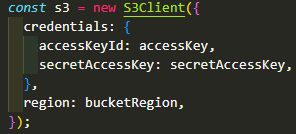
\includegraphics[scale=0.85]{img/actividades/detalles-campanias/objeto-as3.png}
            \caption{Objeto de configuración de Amazon S3.}
            \label{fig:objeto-as3}
        \end{center}
    \end{figure}

Una vez hecha la configuración de Amazon S3, se puede continuar con el procesamiento de los datos.

Como se mencionó anteriormente, el usuario llena un formulario para enviar la información de su solicitud de puntos. El Backend no recibe esta información en formato JSON, como se hizo en el endpoint de inicio de sesión, esta vez la recibe como FormData, y esto es porque el usuario debe subir un archivo, y este formato es el más adecuado para estas situaciones.

Este FormData está formado por dos pares llave/valor: uno con toda la información del formulario (que esta sí está en formato JSON) y otro con el archivo que se va a subir.

El controlador recibe la petición con el FormData y se extraen el ID del usuario, el archivo y la información del formulario. Todo esto, posteriormente, es enviado al servicio.

El servicio es el que se encarga de procesar toda esta información. Primero se trabaja con el archivo, se obtiene la extensión del archivo y se verifica si está entre las permitidas; si no es permitido, se detiene el proceso de subida del archivo y se manda un error, si es permitido, avanza con el proceso. Lo siguiente que se hace es generar una ruta para almacenar la imagen en el bucket, esta ruta tiene la siguiente estructura: ``Campania/idCampania/Pruebas/idUsuario''. Posteriormente se crea un nombre único para el archivo mediante un algoritmo de encriptación que retorna una cadena de caracteres aleatorios, este nombre se anexa al final de la ruta creada anteriormente. Para subir el archivo, se crea un objeto con los parámetros que requiere Amazon S3 para subir un archivo a un bucket, este objeto tiene la siguiente estructura (Ver Figura 10):

    \begin{figure}[H]
        \begin{center}
            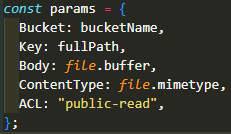
\includegraphics[scale=0.85]{img/actividades/detalles-campanias/params-as3.png}
            \caption{Parámetros para subir un archivo a un bucket.}
            \label{fig:params-as3}
        \end{center}
    \end{figure}

Los parámetros significan lo siguiente: 
    \begin{itemize}
        \item Bucket: Nombre del bucket donde se guardará el archivo.
        \item Key: La ruta donde se guardará el archivo.
        \item Body: El contenido del archivo que se subirá.
        \item ContentType: El formato del archivo.
        \item ACL: La lista de control de acceso para indicar quien podrá ver el archivo y quien no.
    \end{itemize}

Estos parámetros se envían al método correspondiente al objeto que se creó anteriormente en el archivo de configuración, y de esta manera el archivo quedará subido.

El siguiente paso es insertar toda la información en la tabla de la base de datos. Una gran parte de los campos requeridos ya venían en el FormData, por lo que sólo es cuestión de extraerlos y colocarlos en un nuevo objeto que se envía al método encargado de insertar los datos, el único campo nuevo que se debe crear es la URL completa de la imagen, es decir, la URL que contiene tanto el servidor del bucket y la ruta que se creó anteriormente. Este nuevo campo se anexa al objeto y finalmente se envía para insertar esos datos.

Este método retorna el ID del nuevo registro que se creó, este se almacena en una variable para utilizarlo posteriormente. Cabe mencionar que, hasta el momento de la redacción de este reporte, las solicitudes son aceptadas automáticamente, esto por petición de la empresa, lo ideal es que en un futuro las solicitudes pasen por su debido proceso de revisión.

También se deben de insertar los detalles de la solicitud, esto es los productos que se compraron y la cantidad. Al igual que los datos de la inserción anterior, estos detalles también se obtienen del FormData, sólo es cuestión de extraerlos y anexarlos al nuevo objeto que se va a enviar; a este nuevo objeto también se le va a anexar el ID que se almacenó anteriormente.

Para terminar este proceso, sólo falta calcular los nuevos puntos del usuario. Lo primero que se debe hacer es obtener los puntos del usuario, esto se puede hacer utilizando el query que se creó para otro endpoint. El resultado de esta consulta determinará el camino que debe seguir el proceso.

Si el usuario ya tenía puntos se debe realizar una actualización; se toman los puntos que ya tenía y se suman los nuevos que se están solicitando. Realizada esta suma, los nuevos puntos son enviados al método que se encarga de actualizar los puntos.

Si el usuario no tenía puntos se debe realizar una inserción. El primer paso es obtener el día de canje de puntos de la campaña, esto para poder asignarle una vigencia a los nuevos puntos, y después se guarda la fecha actual. A la fecha actual se le adelanta 1 mes, y después se le asigna el día del canje. Por ejemplo: el día del canje es 5, y la fecha de hoy es 20/12/2024, a esta fecha se le adelanta 1 mes por lo que quedaría en 20/01/2025, por último se le establece que el día sea 5 y ahora la fecha quedaría 5/01/2025, esta sería la fecha de vigencia de los puntos.

Esta nueva fecha calculada se anexa al objeto que contiene los datos que se enviarán al método encargado de insertar los puntos en la tabla de la base de datos, y finalmente se insertan los datos.

Como último detalle, todas estas operaciones que se realizaron están dentro de una transacción, por lo que cualquier error que pueda ocurrir en cualquiera de estas detendrá todo el proceso, borrará cualquier operación que se haya realizado y quedará como si no hubiera ocurrido nada.
    \subsection{Interfaz de la sección ``Detalles de las campañas''}
Anteriormente se había mencionado que las Cards donde se mostraban las campañas, cuando el usuario hace clic en ellas, dirigían a una nueva página. Esta nueva página es la sección donde el usuario puede leer toda la información de la campaña que haya seleccionado.

Debido a que esta sección es un poco más grande que otras que se han descrito, se va a separar en dos: el encabezado de la sección y el contenido.

Al igual que en secciones anteriores, mientras se está cargando la información se renderiza el componente ``Skeleton''. Una vez cargada la información, se muestra el contenido normal de la página.
    \subsubsection{Encabezado de la sección ``Detalles de las campañas''}
Cuando el usuario entra a ver la información de una campaña, lo primero que puede ver es el encabezado de la página. En este encabezado se puede ver información básica de la campaña como su nombre, el logo y el banner, además, el usuario también podrá ver la cantidad de puntos que tiene en esa campaña.

Otro componente que podrá ver el usuario es uno llamado ``Breadcrumbs'' que básicamente es un pequeño menú de navegación que muestra toda la ruta de páginas que debió seguir el usuario para llegar a la sección donde se encuentra actualmente.

El encabezado se ve de la siguiente manera (Ver Figura 11):

    \begin{figure}[H]
        \begin{center}
            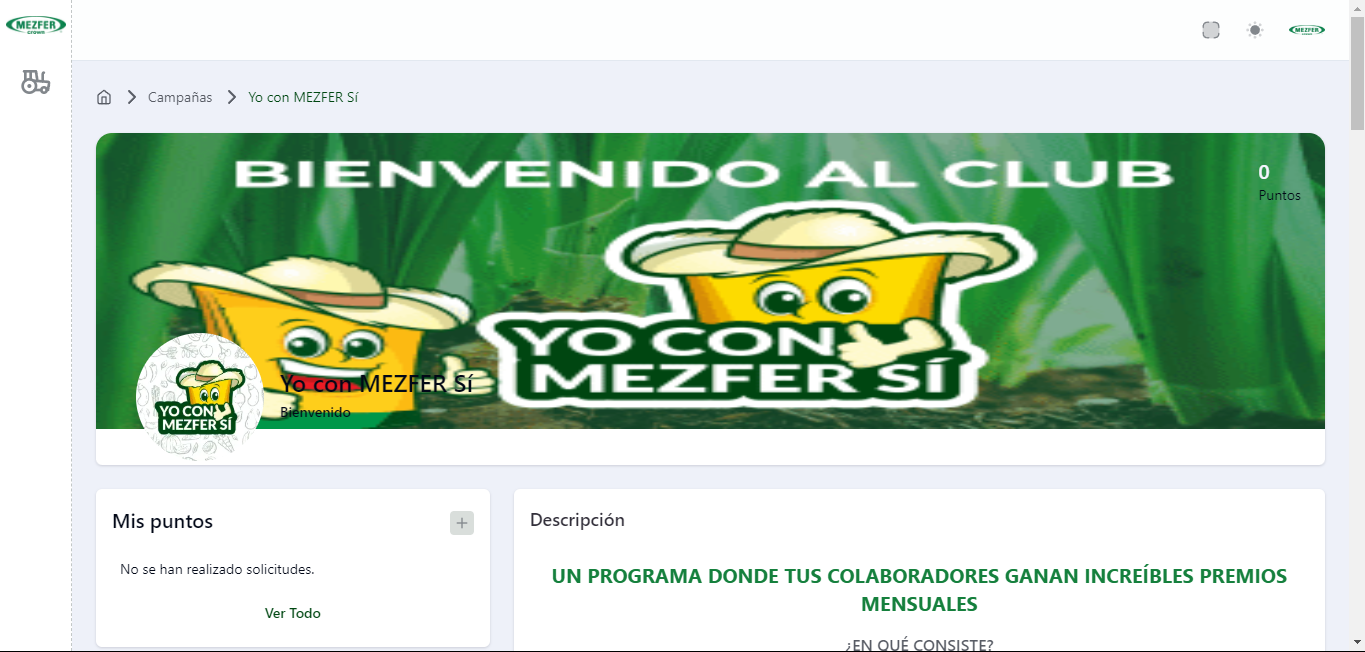
\includegraphics[scale=0.26]{img/actividades/detalles-campanias/encabezado.png}
            \caption{Encabezado de la sección.}
            \label{fig:encabezado}
        \end{center}
    \end{figure}
    \subsubsection{Contenido de la sección ``Detalles de la campaña''}
El contenido de la sección está dividido en 8 Cards diferentes.

La primera Card es la de ``Mis puntos'', el usuario puede ver un historial de las solicitudes de puntos que ha realizado. Si el usuario nunca ha realizado una solicitud de puntos, en la Card sólo le mostrará un mensaje indicándole esto (Ver Figura 12).

    \begin{figure}[H]
        \begin{center}
            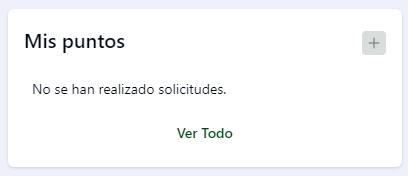
\includegraphics[scale=0.60]{img/actividades/detalles-campanias/card-puntos.png}
            \caption{Card de puntos sin contenido.}
            \label{fig:card-puntos}
        \end{center}
    \end{figure}

Pero si el usuario ya tiene solicitudes hechas, se le mostrarán máximo las últimas 6 solicitudes que ha realizado con información general de la solicitud como la imagen de la evidencia que se subió, la cantidad de puntos que se solicitaron, la fecha en la que se realizó la solicitud y el estatus de la misma (Ver Figura 13).

    \begin{figure}[H]
        \begin{center}
            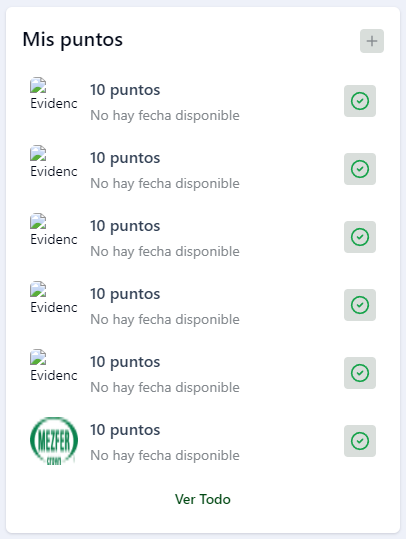
\includegraphics[scale=0.60]{img/actividades/detalles-campanias/card-puntos-contenido.png}
            \caption{Card de puntos con contenido.}
            \label{fig:card-puntos-contenido}
        \end{center}
    \end{figure}

Si el usuario quisiera ver todas las solicitudes que ha realizado, puede presionar el botón que se encuentra en la parte inferior de la Card con la leyenda ``Ver Todo''. Al presionarlo, se mostrará un componente llamado ``Dialog'' y su contenido dependerá de la cantidad de solicitudes hechas; si no hay ninguna, el Dialog sólo contendrá un mensaje indicando esto. (Ver Figura 14).

    \begin{figure}[H]
        \begin{center}
            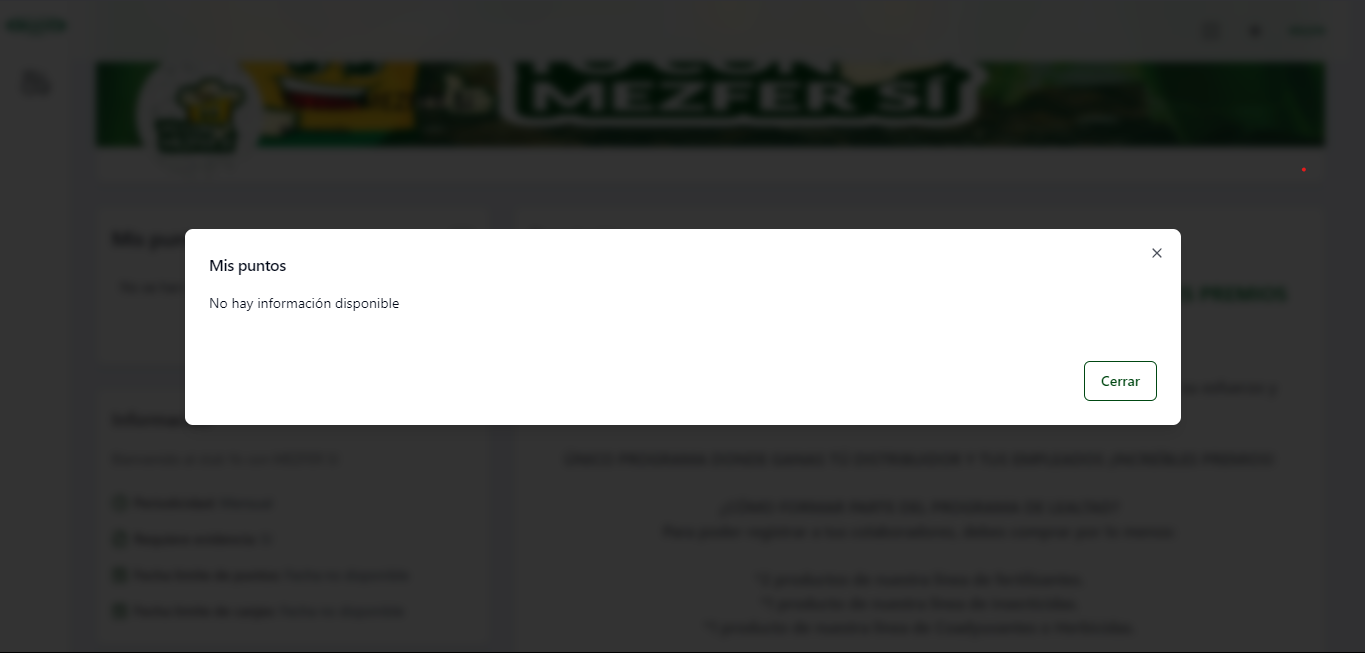
\includegraphics[scale=0.35]{img/actividades/detalles-campanias/dialog-puntos-vacio.png}
            \caption{Dialog de puntos vacío.}
            \label{fig:dialog-puntos-vacio}
        \end{center}
    \end{figure}

Si ya hay solicitudes, el Dialog contendrá una tabla con la información de todas las solicitudes (Ver Figura 15).

    \begin{figure}[H]
        \begin{center}
            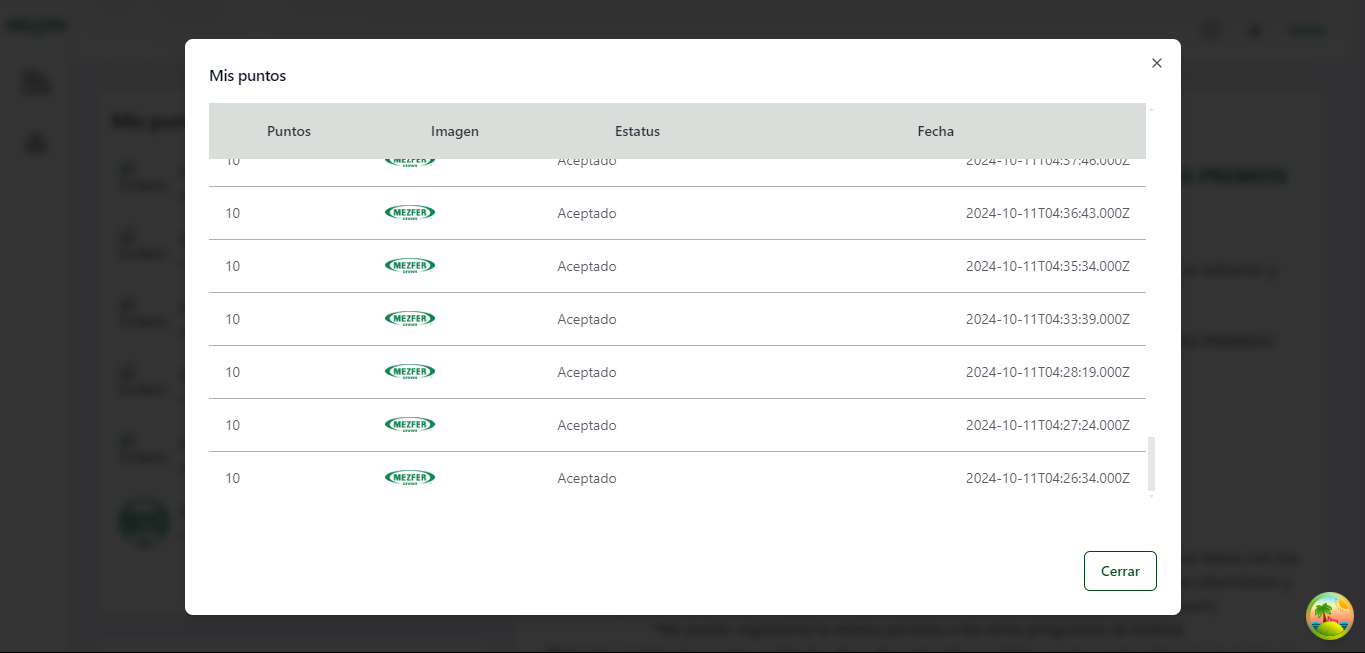
\includegraphics[scale=0.35]{img/actividades/detalles-campanias/dialog-puntos-contenido.png}
            \caption{Dialog de puntos con contenido.}
            \label{fig:dialog-puntos-contenido}
        \end{center}
    \end{figure}

Otra característica importante de esta Card es que permite realizar una solicitud de puntos, esto se hace mediante el botón con un ícono ``+'' que se encuentra en la esquina superior derecha. Al presionarlo, al usuario se le mostrará un Dialog con un formulario para que ingrese toda la información necesaria (Ver Figura 16).

    \begin{figure}[H]
        \begin{center}
            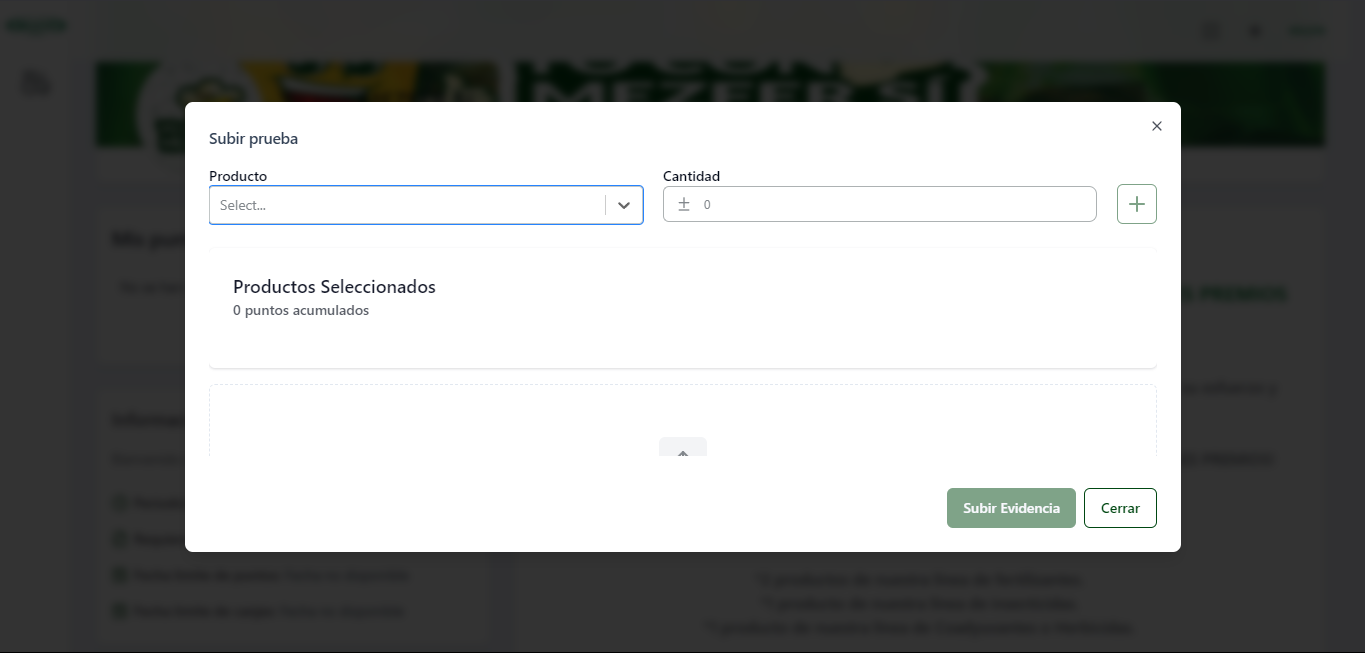
\includegraphics[scale=0.35]{img/actividades/detalles-campanias/dialof-formulario.png}
            \caption{Dialog con formulario para realizar la solicitud.}
            \label{fig:dialog-solicitud}
        \end{center}
    \end{figure}

En la segunda Card se muestra información relevante de la campaña respecto a la periodicidad de esta y las fechas de solicitudes y canjes de los puntos (Ver Figura 17).

    \begin{figure}[H]
        \begin{center}
            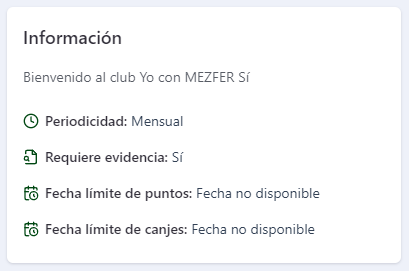
\includegraphics[scale=0.60]{img/actividades/detalles-campanias/card-info-puntos.png}
            \caption{Card con información de la campaña.}
            \label{fig:card-info-campanias}
        \end{center}
    \end{figure}

La tercera Card es donde el usuario puede canjear sus puntos por un premio. Hasta el momento de la redacción de este reporte, esta funcionalidad no está implementada, en la Card sólo se ve un botón pero al presionarlo no ocurre nada (Ver Figura 18).

    \begin{figure}[H]
        \begin{center}
            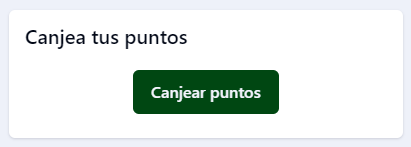
\includegraphics[scale=0.60]{img/actividades/detalles-campanias/card-canje.png}
            \caption{Card de canje de puntos.}
            \label{fig:card-canje}
        \end{center}
    \end{figure}

La cuarta Card muestra los premios que se pueden obtener en la campaña. A simple vista, al usuario se le muestran 6 premios como máximo y sus respectivos detalles como la imagen del premio, el nombre y la cantidad de puntos que se requieren para obtenerlo (Ver Figura 19).

    \begin{figure}[H]
        \begin{center}
            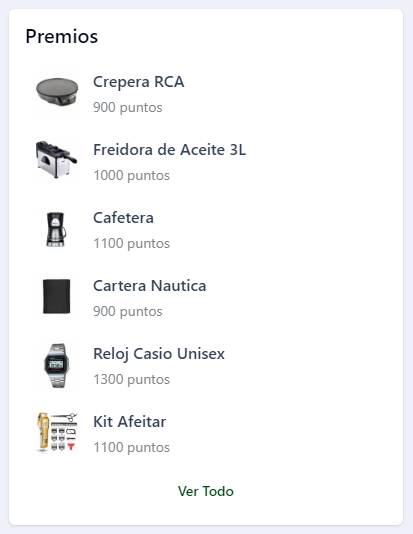
\includegraphics[scale=0.60]{img/actividades/detalles-campanias/card-premios.png}
            \caption{Card con los premios de las campañas.}
            \label{fig:card-premios}
        \end{center}
    \end{figure}

Si el usuario quisiera ver todos los premios disponibles, deberá presionar el botón con la leyenda ``Ver Todo'' que se encuentra en la parte inferior de la Card. Al presionarlo, se mostrará un Dialog con una tabla que contiene la información de todos los premios (Ver Figura 20).

    \begin{figure}[H]
        \begin{center}
            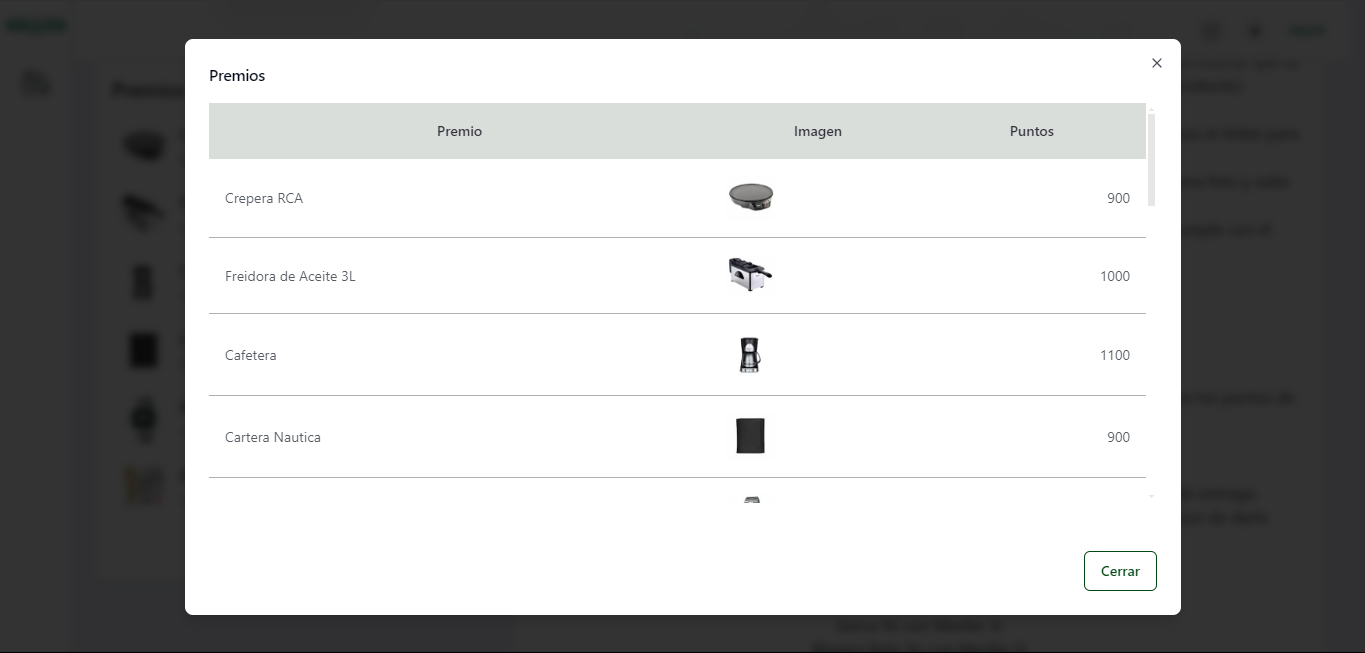
\includegraphics[scale=0.33]{img/actividades/detalles-campanias/dialog-premios.png}
            \caption{Dialog con los premios de la campaña.}
            \label{fig:dialog-premios}
        \end{center}
    \end{figure}

La quinta Card es donde se muestra la descripción de la campaña. En la base de datos, las descripciones están guardadas con información que permite darles el orden y el formato adecuado:
    \begin{itemize}
        \item Número: Este número indica el orden de cada párrafo de la descripción.
        \item Tipo: A cada párrafo se le asigna un tipo como título, subtítulo, información, etc., de esta manera se le puede asignar un color.
    \end{itemize}

Para poder dar un formato aduecuado de todo el texto en la Card, se utilizan arreglos y objetos: en el arreglo se ordenan los párrafos para que el texto tenga sentido, y en el objeto se crean pares llave/valor para que, de acuerdo al tipo de la descripción, se le asigne un color. Otro punto importante es que en la base de datos, el texto de cada párrafo tiene caracteres especiales para indicar los saltos de línea; si este texto se muestra sin darle un formato, estos caracteres también se mostrarán, por lo que es importante que el código pueda identificar estos caracteres y saber que se trata de saltos de línea, y para lograr esto se hace uso de expresiones regulares.

Cubiertos todos estos aspectos, la descripción de la campaña se puede colocar correctamente en la Card (Ver Figura 21).

    \begin{figure}[H]
        \begin{center}
            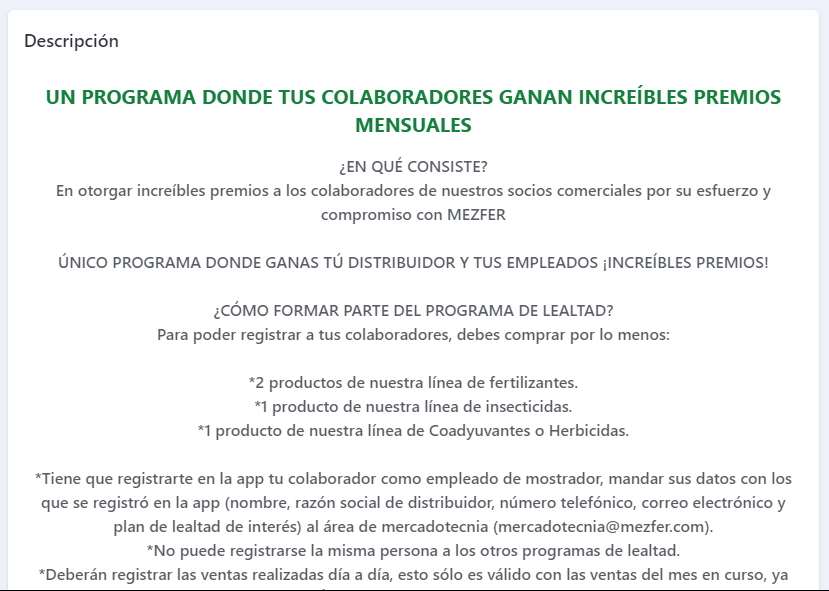
\includegraphics[scale=0.40]{img/actividades/detalles-campanias/card-descripcion.png}
            \caption{Card con la descripcion de la campaña.}
            \label{fig:card-descripcion}
        \end{center}
    \end{figure}

En la sexta Card, se muestra el cuadro de equivalencias de la campaña. Este cuadro de equivalencias muestra todos los productos participantes y la cantidad de puntos que se pueden ganar al comprarlos (Ver Figura 22).

    \begin{figure}[H]
        \begin{center}
            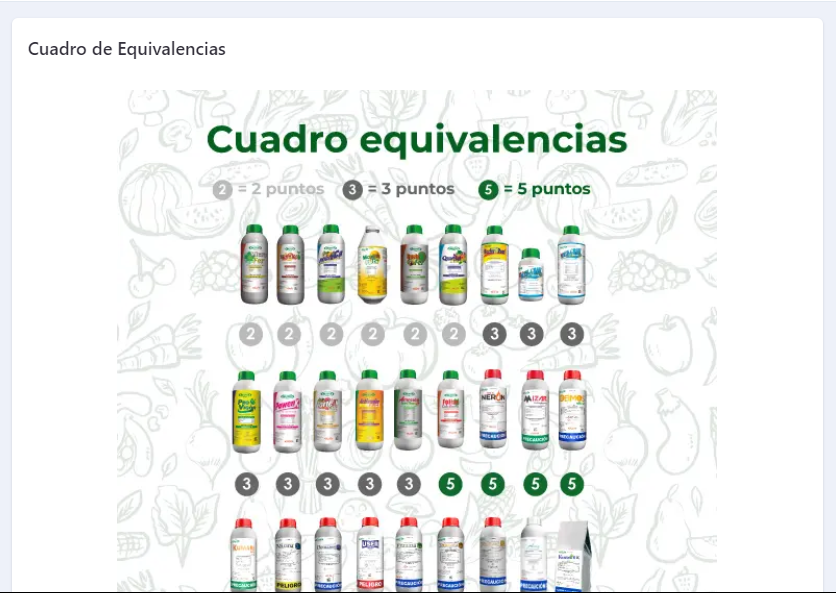
\includegraphics[scale=0.40]{img/actividades/detalles-campanias/card-equivalencias.png}
            \caption{Card con el cuadro de equivalencias.}
            \label{fig:card-equivalencias}
        \end{center}
    \end{figure}

La séptima Card contiene una tabla con los productos que participan en la campaña. Esta tabla está paginada, cada página contiene como máximo 7 productos; también se puede realizar la búsqueda de un producto mediante su nombre con el campo que se encuentra en la parte superior de la tabla, este campo va filtrando el arreglo con todos los productos y retorna las coincidencias que haya con lo que el usuario haya escrito. (Ver Figura 23). 

    \begin{figure}[H]
        \begin{center}
            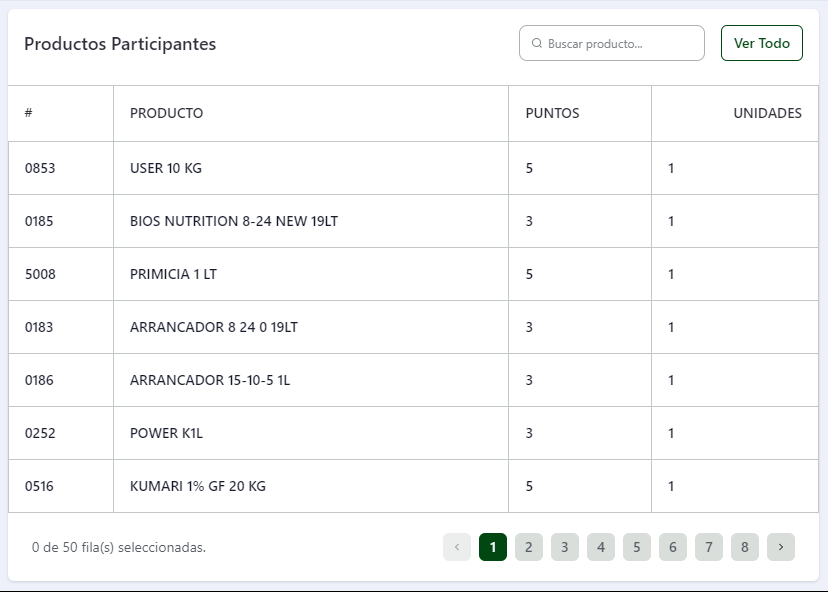
\includegraphics[scale=0.40]{img/actividades/detalles-campanias/card-productos-participantes.png}
            \caption{Card con los productos participantes.}
            \label{fig:card-productos-participantes}
        \end{center}
    \end{figure}

Si el usuario no quisiera navegar por las páginas de la tabla, puede presionar el botón con la leyenda ``Ver Todo'' que se encuentra en la esquina superior derecha. Este botón mostrará un Dialog con una tabla con todos los productos (Ver Figura 24).

    \begin{figure}[H]
        \begin{center}
            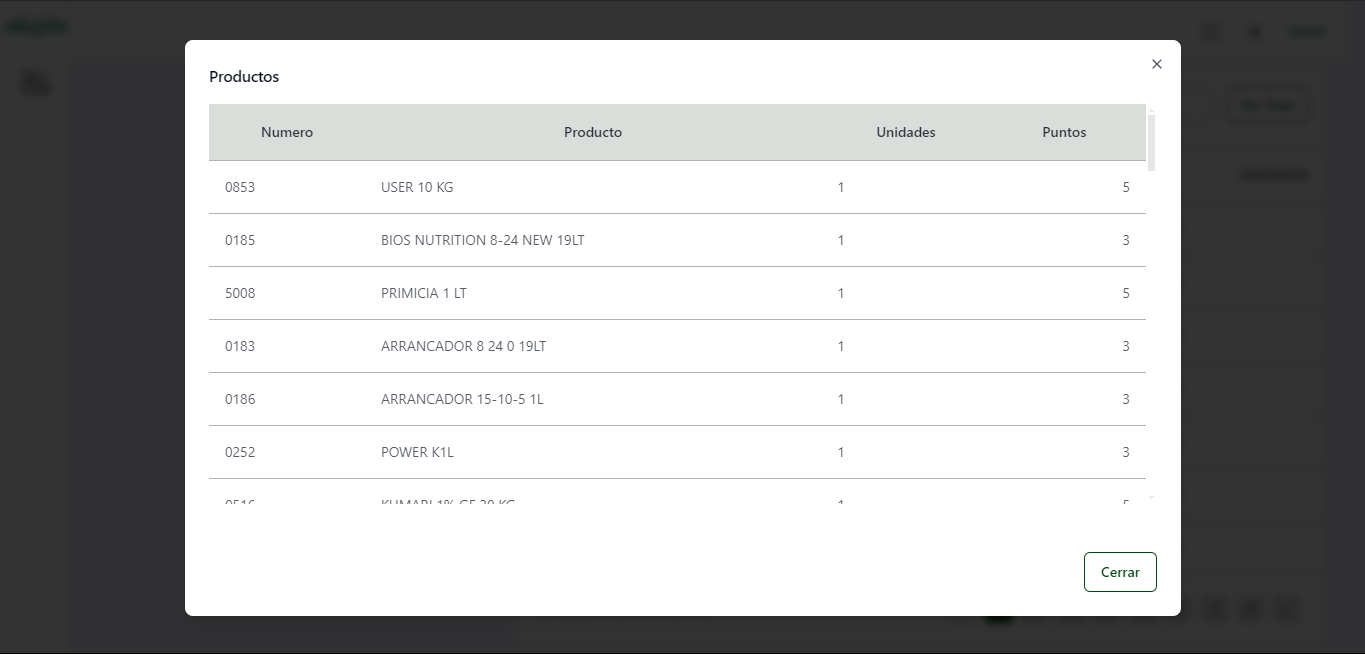
\includegraphics[scale=0.35]{img/actividades/detalles-campanias/dialog-productos-participantes.png}
            \caption{Dialog con los productos de la campaña.}
            \label{fig:dialog-productos-participantes}
        \end{center}
    \end{figure}

La octava y última Card de esta sección contiene una tabla en la que el usuario podrá ver todos los canjes que ha realizado, esta tabla también contiene un campo que permite al usuario buscar cierto canje que haya realizado. Al igual que en Cards anteriores, si el usuario no ha realizado ningún canje, la Card contendrá un mensaje indicándole esto (Ver Figura 25).

    \begin{figure}[H]
        \begin{center}
            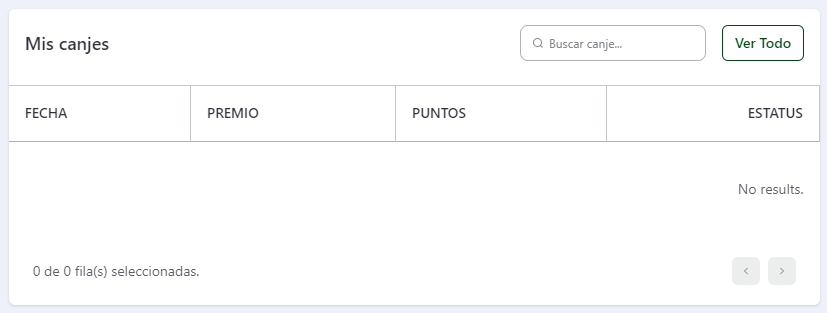
\includegraphics[scale=0.50]{img/actividades/detalles-campanias/card-canjes.png}
            \caption{Card de canjes sin contenido.}
            \label{fig:card-canjes}
        \end{center}
    \end{figure}

Al presionar el botón con la leyenda ``Ver Todo'' que se encuentra en la esquina superior derecha, al usuario se le mostrará un Dialog con una tabla sin paginación con todos los canjes que ha realizado. En este caso, como no hay información que mostrar, sólo se mostrará un mensaje indicando esto (Ver Figura 26).

    \begin{figure}[H]
        \begin{center}
            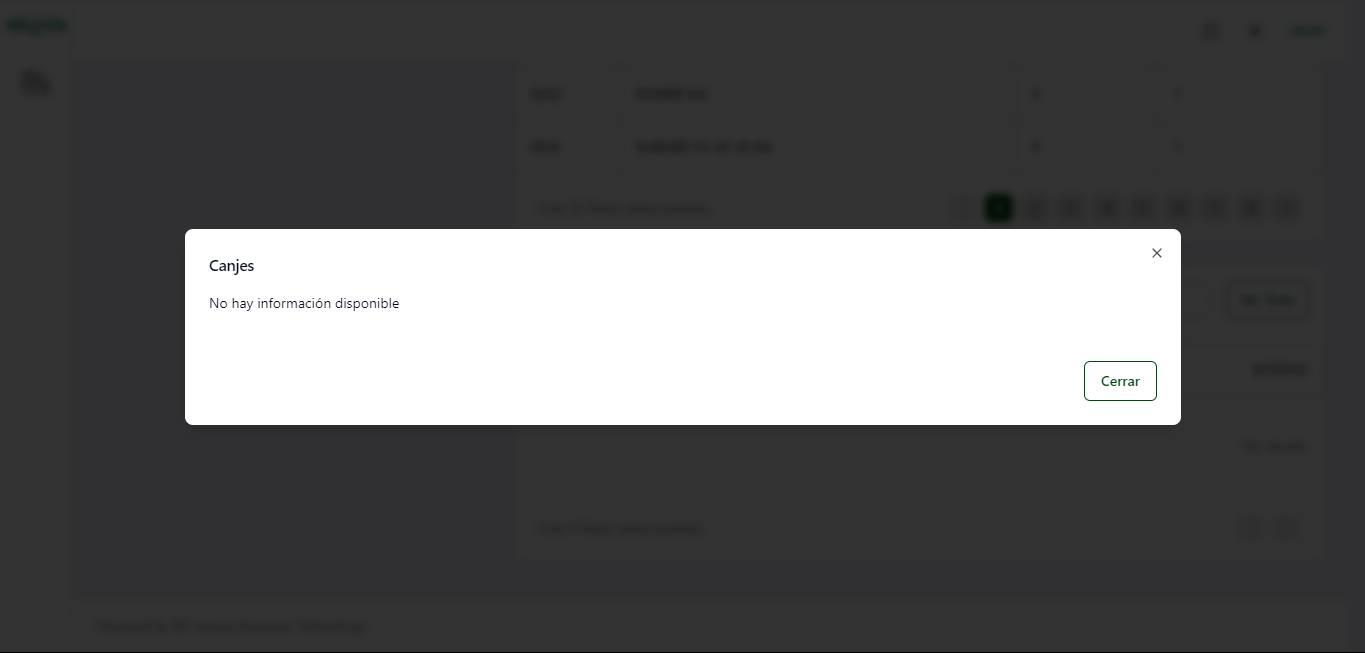
\includegraphics[scale=0.35]{img/actividades/detalles-campanias/dialog-canjes-vacio.png}
            \caption{Dialog de canjes sin contenido.}
            \label{fig:dialog-canjes-vacio}
        \end{center}
    \end{figure}

Si ya hay canjes realizados, el usuario podrá ver todos los detalles de estos (Ver Figura 27).

    \begin{figure}[H]
        \begin{center}
            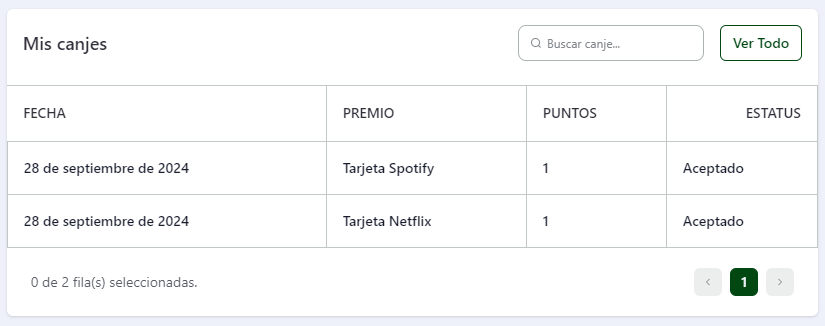
\includegraphics[scale=0.50]{img/actividades/detalles-campanias/card-canjes-contenido.png}
            \caption{Card de canjes con contenido.}
            \label{fig:card-canjes-contenido}
        \end{center}
    \end{figure}

Y esta misma información la podrá ver en el Dialog con una tabla sin paginación que se muestra al presionar el botón ``Ver Todo'' (Ver Figura 28).

\begin{figure}[H]
    \begin{center}
        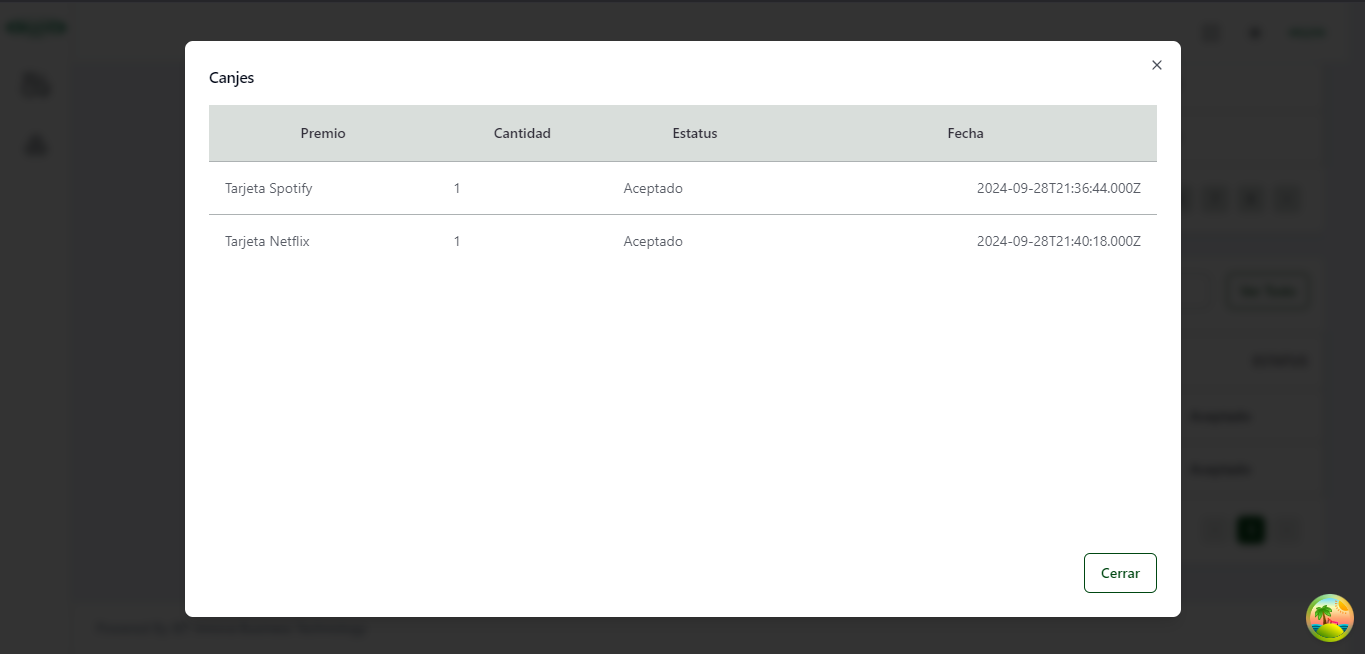
\includegraphics[scale=0.32]{img/actividades/detalles-campanias/dialog-canjes-contenido.png}
        \caption{Dialog de canjes con contenido.}
        \label{fig:dialog-canjes-contenido}
    \end{center}
\end{figure}
    \section{Cambios generales en el Frontend de los clientes}
Los cambios que se realizaron en el Frontend de los clientes son relacionados al código y a algunos componentes.

En cuanto al código, se cambió la manera en las que se estaban realizando las peticiones HTTP. Las peticiones se estaban realizando de manera repetida en diferentes partes del código, por lo que se decidió realizarlas desde un mismo lugar y la información que se obtuviera se pasaría a los diferentes componentes que la necesitaran. Además, como la misma estructura de código se repetía, se decidió crear un hook para realizar las peticiones; ahora en vez de escribir el mismo código múltiples veces, simplemente se manda a llamar un método que solicita una URL y el tipo de petición.

Otro cambio importante que se realizó fue en los componentes. Algunos componentes como tablas, Dialogs y Cards se estaban creando por cada sección que los ocupara y esto sólo hacía que el tamaño del proyecto estuviera aumentando, es por eso que se decidió crear componentes reutilizables, esto permitió que en un solo archivo estuviera el códgio general de cada componente y sólo se les pasaba la información que se quisiera mostrar en ellos.


    \section{Dashboard de los administradores}
